% Options for packages loaded elsewhere
\PassOptionsToPackage{unicode}{hyperref}
\PassOptionsToPackage{hyphens}{url}
\PassOptionsToPackage{dvipsnames,svgnames,x11names}{xcolor}
%
\documentclass[
  11,
  a4paper,
]{article}

\usepackage{amsmath,amssymb}
\usepackage{setspace}
\usepackage{iftex}
\ifPDFTeX
  \usepackage[T1]{fontenc}
  \usepackage[utf8]{inputenc}
  \usepackage{textcomp} % provide euro and other symbols
\else % if luatex or xetex
  \usepackage{unicode-math}
  \defaultfontfeatures{Scale=MatchLowercase}
  \defaultfontfeatures[\rmfamily]{Ligatures=TeX,Scale=1}
\fi
\usepackage{lmodern}
\ifPDFTeX\else  
    % xetex/luatex font selection
  \setmainfont[Numbers=Lowercase,Numbers=Proportional]{Times New Roman}
\fi
% Use upquote if available, for straight quotes in verbatim environments
\IfFileExists{upquote.sty}{\usepackage{upquote}}{}
\IfFileExists{microtype.sty}{% use microtype if available
  \usepackage[]{microtype}
  \UseMicrotypeSet[protrusion]{basicmath} % disable protrusion for tt fonts
}{}
\makeatletter
\@ifundefined{KOMAClassName}{% if non-KOMA class
  \IfFileExists{parskip.sty}{%
    \usepackage{parskip}
  }{% else
    \setlength{\parindent}{0pt}
    \setlength{\parskip}{6pt plus 2pt minus 1pt}}
}{% if KOMA class
  \KOMAoptions{parskip=half}}
\makeatother
\usepackage{xcolor}
\usepackage[top=15mm,left=22.5mm,right=22.5mm,bottom=15mm]{geometry}
\setlength{\emergencystretch}{3em} % prevent overfull lines
\setcounter{secnumdepth}{-\maxdimen} % remove section numbering
% Make \paragraph and \subparagraph free-standing
\ifx\paragraph\undefined\else
  \let\oldparagraph\paragraph
  \renewcommand{\paragraph}[1]{\oldparagraph{#1}\mbox{}}
\fi
\ifx\subparagraph\undefined\else
  \let\oldsubparagraph\subparagraph
  \renewcommand{\subparagraph}[1]{\oldsubparagraph{#1}\mbox{}}
\fi


\providecommand{\tightlist}{%
  \setlength{\itemsep}{0pt}\setlength{\parskip}{0pt}}\usepackage{longtable,booktabs,array}
\usepackage{calc} % for calculating minipage widths
% Correct order of tables after \paragraph or \subparagraph
\usepackage{etoolbox}
\makeatletter
\patchcmd\longtable{\par}{\if@noskipsec\mbox{}\fi\par}{}{}
\makeatother
% Allow footnotes in longtable head/foot
\IfFileExists{footnotehyper.sty}{\usepackage{footnotehyper}}{\usepackage{footnote}}
\makesavenoteenv{longtable}
\usepackage{graphicx}
\makeatletter
\def\maxwidth{\ifdim\Gin@nat@width>\linewidth\linewidth\else\Gin@nat@width\fi}
\def\maxheight{\ifdim\Gin@nat@height>\textheight\textheight\else\Gin@nat@height\fi}
\makeatother
% Scale images if necessary, so that they will not overflow the page
% margins by default, and it is still possible to overwrite the defaults
% using explicit options in \includegraphics[width, height, ...]{}
\setkeys{Gin}{width=\maxwidth,height=\maxheight,keepaspectratio}
% Set default figure placement to htbp
\makeatletter
\def\fps@figure{htbp}
\makeatother
% definitions for citeproc citations
\NewDocumentCommand\citeproctext{}{}
\NewDocumentCommand\citeproc{mm}{%
  \begingroup\def\citeproctext{#2}\cite{#1}\endgroup}
\makeatletter
 % allow citations to break across lines
 \let\@cite@ofmt\@firstofone
 % avoid brackets around text for \cite:
 \def\@biblabel#1{}
 \def\@cite#1#2{{#1\if@tempswa , #2\fi}}
\makeatother
\newlength{\cslhangindent}
\setlength{\cslhangindent}{1.5em}
\newlength{\csllabelwidth}
\setlength{\csllabelwidth}{3em}
\newenvironment{CSLReferences}[2] % #1 hanging-indent, #2 entry-spacing
 {\begin{list}{}{%
  \setlength{\itemindent}{0pt}
  \setlength{\leftmargin}{0pt}
  \setlength{\parsep}{0pt}
  % turn on hanging indent if param 1 is 1
  \ifodd #1
   \setlength{\leftmargin}{\cslhangindent}
   \setlength{\itemindent}{-1\cslhangindent}
  \fi
  % set entry spacing
  \setlength{\itemsep}{#2\baselineskip}}}
 {\end{list}}
\usepackage{calc}
\newcommand{\CSLBlock}[1]{\hfill\break\parbox[t]{\linewidth}{\strut\ignorespaces#1\strut}}
\newcommand{\CSLLeftMargin}[1]{\parbox[t]{\csllabelwidth}{\strut#1\strut}}
\newcommand{\CSLRightInline}[1]{\parbox[t]{\linewidth - \csllabelwidth}{\strut#1\strut}}
\newcommand{\CSLIndent}[1]{\hspace{\cslhangindent}#1}

\usepackage{lscape}
\newcommand{\blandscape}{\begin{landscape}}
\newcommand{\elandscape}{\end{landscape}}
\makeatletter
\@ifpackageloaded{caption}{}{\usepackage{caption}}
\AtBeginDocument{%
\ifdefined\contentsname
  \renewcommand*\contentsname{Table of contents}
\else
  \newcommand\contentsname{Table of contents}
\fi
\ifdefined\listfigurename
  \renewcommand*\listfigurename{List of Figures}
\else
  \newcommand\listfigurename{List of Figures}
\fi
\ifdefined\listtablename
  \renewcommand*\listtablename{List of Tables}
\else
  \newcommand\listtablename{List of Tables}
\fi
\ifdefined\figurename
  \renewcommand*\figurename{Figure}
\else
  \newcommand\figurename{Figure}
\fi
\ifdefined\tablename
  \renewcommand*\tablename{Table}
\else
  \newcommand\tablename{Table}
\fi
}
\@ifpackageloaded{float}{}{\usepackage{float}}
\floatstyle{ruled}
\@ifundefined{c@chapter}{\newfloat{codelisting}{h}{lop}}{\newfloat{codelisting}{h}{lop}[chapter]}
\floatname{codelisting}{Listing}
\newcommand*\listoflistings{\listof{codelisting}{List of Listings}}
\makeatother
\makeatletter
\makeatother
\makeatletter
\@ifpackageloaded{caption}{}{\usepackage{caption}}
\@ifpackageloaded{subcaption}{}{\usepackage{subcaption}}
\makeatother
\ifLuaTeX
  \usepackage{selnolig}  % disable illegal ligatures
\fi
\usepackage{bookmark}

\IfFileExists{xurl.sty}{\usepackage{xurl}}{} % add URL line breaks if available
\urlstyle{same} % disable monospaced font for URLs
\hypersetup{
  pdftitle={The genomic landscape of Acute Respiratory Distress Syndrome: a meta-analysis by information content of genome-wide studies of the host response.},
  colorlinks=true,
  linkcolor={blue},
  filecolor={Maroon},
  citecolor={Blue},
  urlcolor={Blue},
  pdfcreator={LaTeX via pandoc}}

\title{The genomic landscape of Acute Respiratory Distress Syndrome: a
meta-analysis by information content of genome-wide studies of the host
response.}
\author{}
\date{}

\begin{document}
\maketitle

\setstretch{1.5}
Jonathan E Millar\textsuperscript{1,2}, Sara
Clohisey-Hendry\textsuperscript{1,2}, Megan McMannus\textsuperscript{1},
Marie Zechner\textsuperscript{1}, Bo Wang\textsuperscript{1}, Nick
Parkinson\textsuperscript{1}, Melissa Jungnickel\textsuperscript{1},
Nureen Mohamad Zaki\textsuperscript{1}, Erola
Pairo-Castineira\textsuperscript{1,2}, Konrad
Rawlik\textsuperscript{1,2}, Joshua Rogers\textsuperscript{1}, Clark D
Russell\textsuperscript{2}, Lieuwe DJ Bos\textsuperscript{3}, Nuala J
Meyer\textsuperscript{4}, Carolyn Calfee\textsuperscript{5}, Daniel F
McAuley\textsuperscript{6}, Manu Shankar-Hari\textsuperscript{2} and J
Kenneth Baillie\textsuperscript{1,2}

\begin{enumerate}
\def\labelenumi{\arabic{enumi}.}
\tightlist
\item
  Roslin Institute, University of Edinburgh, Edinburgh, United Kingdom.
\item
  Baillie-Gifford Pandemic Science Hub, Centre for Inflammation
  Research, University of Edinburgh, Edinburgh, United Kingdom.
\item
  Intensive Care, Amsterdam UMC-location AMC, University of Amsterdam,
  Amsterdam, The Netherlands.
\item
  Division of Pulmonary, Allergy, and Critical Care, University of
  Pennsylvania Perelman School of Medicine, Philadelphia, Pennsylvania,
  USA.
\item
  Division of Pulmonary, Critical Care, Allergy \& Sleep Medicine,
  Department of Medicine, University of California San Francisco, San
  Francisco, California, USA.
\item
  Wellcome-Wolfson Institute for Experimental Medicine, Queen's
  University Belfast, Belfast, United Kingdom.
\end{enumerate}

\newpage

\subsection{Abstract}\label{abstract}

Acute respiratory distress syndrome (ARDS) is a clinically defined
syndrome of acute hypoxaemic respiratory failure secondary to
non-cardiogenic pulmonary oedema. It arises from a diverse set of
triggers and encompasses marked biological heterogeneity, complicating
efforts to develop effective therapies. An extensive body of recent work
(including transcriptomics, proteomics, and genome-wide association
studies) has sought to identify proteins/genes implicated in ARDS
pathogenesis. These diverse studies have not been systematically
collated and interpreted.

To solve this, we performed a systematic review and computational
integration of existing omics data implicating host response pathways in
ARDS pathogenesis. We identified 40 unbiased studies reporting
associations, correlations other links with 7000 named protein-coding
genes, from 6,856 ARDS patients.

We used meta-analysis by information content (MAIC) to integrate and
evaluate these data, ranking over 7,000 genes and weighting cumulative
evidence for association. Functional enrichment of strongly-supported
genes revealed cholesterol metabolism, endothelial dysfunction, innate
immune activation and neutrophil degranulation as key processes. We
identify 51 hub genes, most of which are potential therapeutic targets.
To explore biological heterogeneity, we conducted a separate analysis of
ARDS severity/outcomes, revealing distinct gene associations and tissue
specificity. Our large-scale integration of existing omics data in ARDS
enhances understanding of the genomic landscape by synthesising decades
of data from diverse sources. The findings will help researchers refine
hypotheses, select candidate genes for functional validation, and
identify potential therapeutic targets and repurposing opportunities.
Our study and the publicly available computational framework represent
an open, evolving platform for interpretation of ARDS genomic data.

\newpage

\subsection{Introduction}\label{introduction}

The acute respiratory distress syndrome (ARDS) is clinically defined as
acute hypoxaemic respiratory failure due to non-cardiogenic pulmonary
oedema\textsuperscript{1}. It occurs following a variety of insults;
pulmonary and extra-pulmonary. While this definition has been useful in
identifying patients at risk of serious morbidity and
death\textsuperscript{2}, it overlooks the underlying biology and masks
heterogeneity\textsuperscript{3}. Arguably, this has contributed to
limited success in developing therapeutics\textsuperscript{4}. In
contrast, a biological definition of ARDS may provide the lever
necessary for future drug discovery\textsuperscript{5}.

Functional genomics technologies enable hypothesis-free disease
characterisation at unprecedented resolution. The emergence of
coronavirus disease 2019 (COVID-19) has provided an opportunity to test
genetic approaches to drug discovery in a homogeneous subset of ARDS
patients. A notable success is the finding that baricitinib, a Janus
kinase inhibitor, reduces mortality in patients hospitalised with
COVID-19\textsuperscript{6}. \emph{A priori} support for
baricitinib\textsuperscript{7} was greatly enhanced following the
discovery of a causal link between elevated tyrosine kinase 2 (TYK2)
expression and severe COVID-19 in genome-wide association studies
(GWAS)\textsuperscript{8}. The availability of comparable omics data for
non-COVID ARDS is limited.

An unresolved challenge is how large omics data can be effectively
exploited\textsuperscript{9}. Specifically, how can we combine data from
heterogeneous sources to derive new insights or recalibrate our
understanding in the light of new data? We have proposed meta-analysis
by information content (MAIC) as a data-driven, algorithmic, method for
combining gene lists from diverse sources\textsuperscript{10}. MAIC is
agnostic to the quality or methodology of the sources and combines
ranked or un-ranked gene sets by calculating weights for each list and
gene, and iteratively updating them to converge on a ranked meta-list.
We have successfully applied MAIC to host-genomics studies of Influenza
A\textsuperscript{10} and coronavirus infection\textsuperscript{8,11},
and shown that it out-performs existing algorithms when combining ranked
and un-ranked lists obtained from heterogeneous
sources\textsuperscript{12}.

In this work, we present a living meta-analysis by information content
of ARDS host genomics studies. This serves as an open-source resource
for gene prioritisation, functional genomics, and drug target discovery.
An interactive interface can be accessed at
\url{https://baillielab.net/maic/ards}, alongside a complementary
\href{https://github.com/baillielab/ARDSMAICr}{R package}.

\newpage

\subsection{Results}\label{results}

\paragraph{Systematic review}\label{systematic-review}

We first conducted a systematic review of existing genome-wide studies,
which reported associations between genes, transcripts, or proteins and
ARDS susceptibility, severity, survival, or phenotype. Our search
yielded 8,937 unique citations (Fig. S1). We retrieved 74 articles for
full-text evaluation and included 40 in our
meta-analysis\textsuperscript{13--52}. These 40 studies produced 44
unique gene lists (22 transcriptomic, 13 proteomic, and 9 based on
genome-wide association studies (GWAS); see Table~\ref{tbl-tab1}). Three
studies reported results from multiple
methodologies\textsuperscript{33,38,44}, and several used more than one
tissue type\textsuperscript{18,21,32}. Excluding GWAS, 14 gene lists
(40\%) were derived from lung or airways samples, and 21 (60\%) from
blood. We could not retrieve one gene list\textsuperscript{26}. No
whole-genome sequencing GWAS were found, and only 36\% (n=8) of
transcriptomic lists used next-generation sequencing techniques. The
earliest included study was published in 2004\textsuperscript{18},
however, almost half (n=19, 47.5\%) were published in the last 5 years.

Most studies aimed to identify genes or proteins associated with ARDS
susceptibility (n=27, 67.5\%). The remainder examined associations with
survival (n=6, 15\%), sub-phenotype (n=4, 10\%), disease progression
(n=2, 5\%), or severity (n=1, 2.5\%). In total, studies included 6,856
patients with ARDS.

\paragraph{Meta-analysis by information content
(MAIC)}\label{meta-analysis-by-information-content-maic}

We analysed all 43 available gene lists using MAIC. Lists were
categorised by method (i.e., GWAS, transcriptomics, and proteomics) and
technique (e.g., RNA-seq, mass spectrometry; see Table 1). In total, we
ranked 7,085 unique genes (or SNPs), with a median of 27 genes per gene
list (range 1-4,954). The top 100 ranked genes are summarized in
Figure~\ref{fig-fig1}. Most genes were found in a single category
(n=5,866, 82.8\%); only 157 (2.2\%) were identified in ≥ 3 categories,
with the maximum number of categories supporting a gene being 5
(Figure~\ref{fig-fig1}). Similarly, few genes (n=362, 5.1\%) were
identified by more than one method, with only \emph{AKR1B10},
\emph{HINT1}, \emph{HSPG2}, \emph{S100A11}, and \emph{SLC18A1} present
in transcriptomic, proteomic, and GWAS-based lists.

To prioritise genes for further investigation, we used the unit
invariant knee method\textsuperscript{53} to identify the inflection
point in the MAIC score curve. This prioritised 1,306 genes with scores
above this point (Figure~\ref{fig-fig1}). These genes were more likely
to be found in ≥ 2 lists or categories and by more than one method
(Figure~\ref{fig-fig1}).

\begin{figure}

\centering{

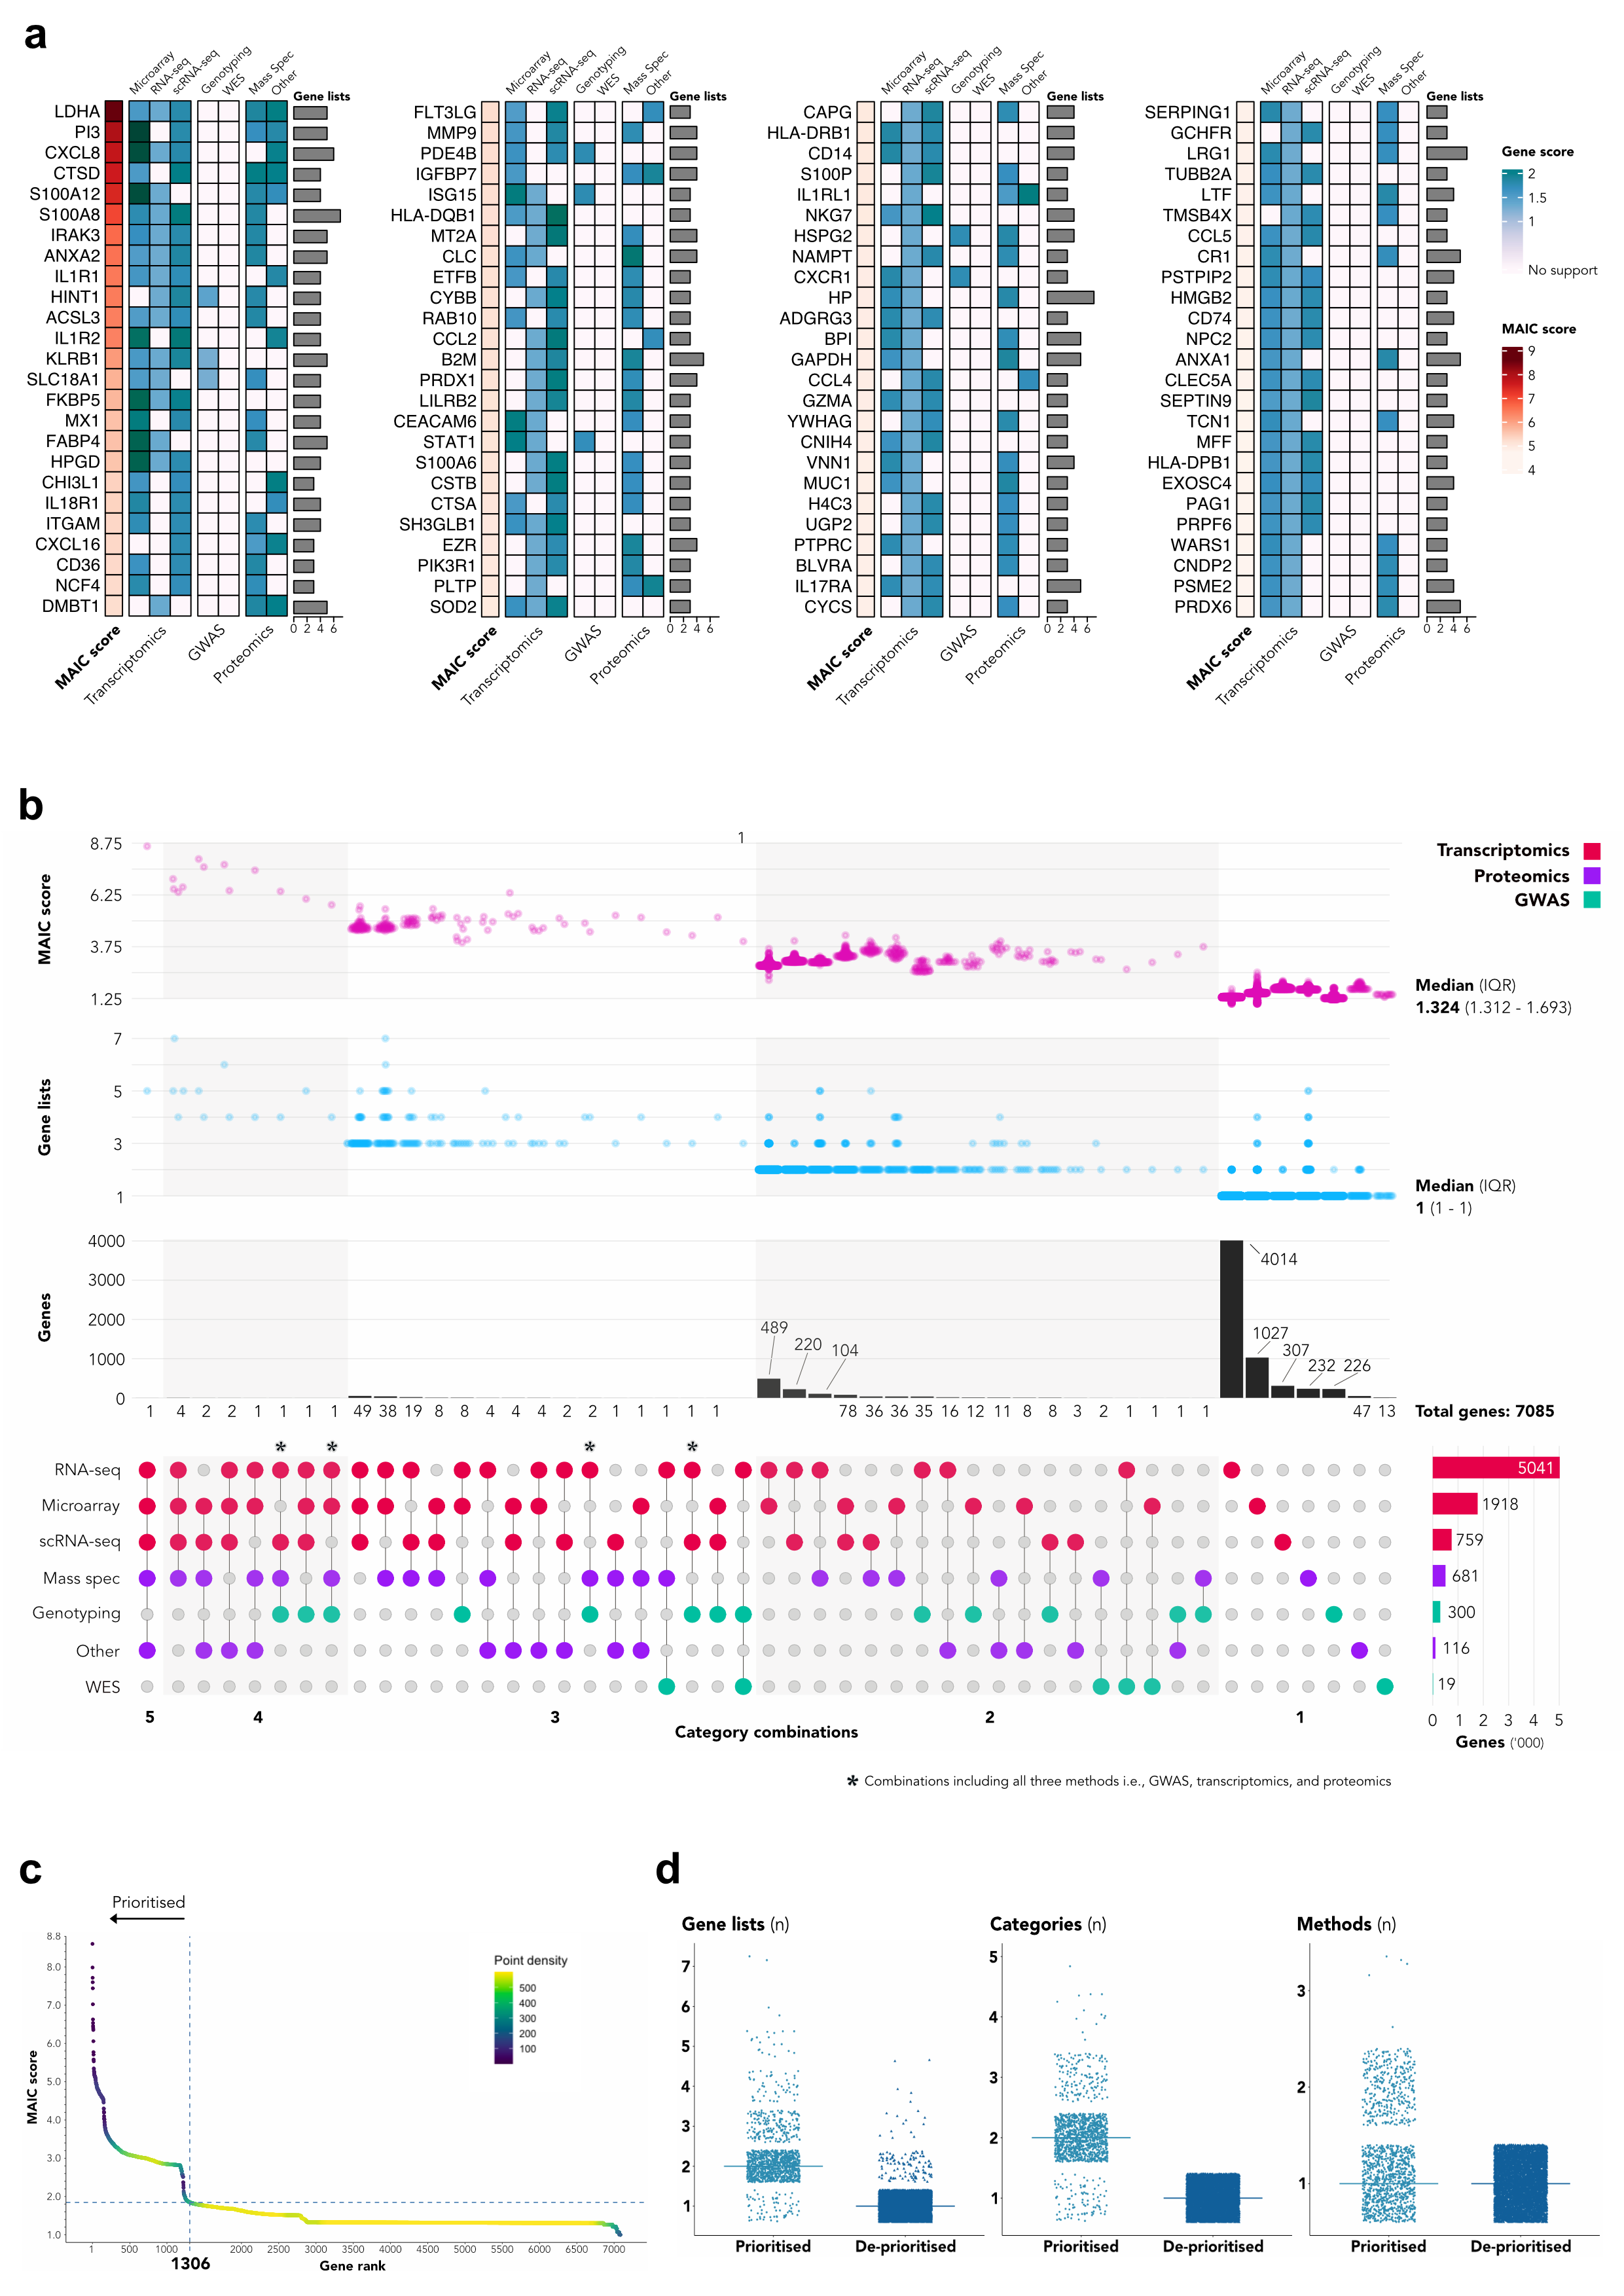
\includegraphics{./img/Figure_1.png}

}

\caption{\label{fig-fig1}\textbf{Meta-analysis by information content}.
(a) Heatmap of top 100 ranked genes showing MAIC score, highest score
per category, and number of supporting lists. (b) UpSet plot of ranked
genes showing total numbers for each category combination, MAIC score
distribution, and supporting lists. (c) Gene prioritisation using the
Unit Invariant Knee method. Intersection of lines identifies elbow point
of best-fit curve. 1,306 genes in the upper left quadrant were
prioritied. (d) Strip plots comparing number of lists , categories, and
methods per gene between prioritised and deprioritised sets.}

\end{figure}%

To assess the influence of individual lists, we calculated the total
MAIC score (totMS), reflecting the sum of gene scores across each list
(Fig. S2), and the contributing total MAIC score (ctotMS), measuring the
sum of each lists gene scores which contribute to a gene's overall MAIC
score. To obtain relative values, we divided the tot/MS/ctotMS for each
list by the total across all included lists. This demonstrated that only
10 lists (from 9 studies) contributed \textgreater1\% by either metric
(Tab. S2). Notably, the RNA-seq list from Sarma et
al.\textsuperscript{44} accounts for \textgreater50\%, a function of its
length. To account for this, we normalised totMS/ctotMS by the number of
genes per list; along with the proportion of replicated genes in each
list, this provides an alternative perspective, with several proteomic
studies ranking highly (Fig. S2).

\paragraph{Comparison with existing ARDS sources and
COVID-19}\label{comparison-with-existing-ards-sources-and-covid-19}

To place our meta-analysis results in context, we evaluated the overlap
between the genes prioritised by MAIC and those from two established
resources: BioLitMine\textsuperscript{54}, using an ARDS MeSH search,
and the ARDS Database of Genes\textsuperscript{55} (Fig. S3a and Fig.
S3c). A search using BioLitMine, identified 271 ARDS-associated genes,
of which 142 (52.4\%) were present in our analysis. Almost half of the
overlapping genes (n = 63, 44.4\%) ranked within our prioritised set
(Tab. S3).

\newpage

\blandscape

\begin{longtable}[]{@{}
  >{\raggedright\arraybackslash}p{(\columnwidth - 16\tabcolsep) * \real{0.0676}}
  >{\raggedright\arraybackslash}p{(\columnwidth - 16\tabcolsep) * \real{0.2162}}
  >{\raggedright\arraybackslash}p{(\columnwidth - 16\tabcolsep) * \real{0.1351}}
  >{\raggedright\arraybackslash}p{(\columnwidth - 16\tabcolsep) * \real{0.1081}}
  >{\raggedright\arraybackslash}p{(\columnwidth - 16\tabcolsep) * \real{0.0676}}
  >{\raggedright\arraybackslash}p{(\columnwidth - 16\tabcolsep) * \real{0.1149}}
  >{\raggedright\arraybackslash}p{(\columnwidth - 16\tabcolsep) * \real{0.1081}}
  >{\raggedright\arraybackslash}p{(\columnwidth - 16\tabcolsep) * \real{0.0811}}
  >{\raggedright\arraybackslash}p{(\columnwidth - 16\tabcolsep) * \real{0.1014}}@{}}
\caption{Summary of studies and gene lists included in the systematic
review}\label{tbl-tab1}\tabularnewline
\toprule\noalign{}
\begin{minipage}[b]{\linewidth}\raggedright
\textbf{Year}
\end{minipage} & \begin{minipage}[b]{\linewidth}\raggedright
\textbf{Study}
\end{minipage} & \begin{minipage}[b]{\linewidth}\raggedright
\textbf{Focus}
\end{minipage} & \begin{minipage}[b]{\linewidth}\raggedright
\textbf{Definition}
\end{minipage} & \begin{minipage}[b]{\linewidth}\raggedright
\textbf{N}\textsuperscript{a}
\end{minipage} & \begin{minipage}[b]{\linewidth}\raggedright
\textbf{Method}
\end{minipage} & \begin{minipage}[b]{\linewidth}\raggedright
\textbf{Technique}
\end{minipage} & \begin{minipage}[b]{\linewidth}\raggedright
\textbf{Tissue}
\end{minipage} & \begin{minipage}[b]{\linewidth}\raggedright
\textbf{Cell type}
\end{minipage} \\
\midrule\noalign{}
\endfirsthead
\toprule\noalign{}
\begin{minipage}[b]{\linewidth}\raggedright
\textbf{Year}
\end{minipage} & \begin{minipage}[b]{\linewidth}\raggedright
\textbf{Study}
\end{minipage} & \begin{minipage}[b]{\linewidth}\raggedright
\textbf{Focus}
\end{minipage} & \begin{minipage}[b]{\linewidth}\raggedright
\textbf{Definition}
\end{minipage} & \begin{minipage}[b]{\linewidth}\raggedright
\textbf{N}\textsuperscript{a}
\end{minipage} & \begin{minipage}[b]{\linewidth}\raggedright
\textbf{Method}
\end{minipage} & \begin{minipage}[b]{\linewidth}\raggedright
\textbf{Technique}
\end{minipage} & \begin{minipage}[b]{\linewidth}\raggedright
\textbf{Tissue}
\end{minipage} & \begin{minipage}[b]{\linewidth}\raggedright
\textbf{Cell type}
\end{minipage} \\
\midrule\noalign{}
\endhead
\bottomrule\noalign{}
\endlastfoot
2022 & Batra\textsuperscript{13} & Survival & Berlin & 24 & Proteomics &
Other & Blood & \\
& Mirchandani\textsuperscript{38} & ARDS vs.~non-ARDS & Berlin & 22 &
Proteomics & Mass Spec & Blood & Monocytes \\
& & & & & Transcriptomics & Microarray & Blood & Monocytes \\
& Sarma\textsuperscript{44} & Sub-phenotype & Berlin & 41 & Proteomics &
Other & TA & \\
& & & & & Transcriptomics & RNA-seq & TA & \\
& & & & & Transcriptomics & scRNA-Seq & TA & Immune cells \\
& Zhang\textsuperscript{51} & ARDS vs.~non-ARDS & AECC & 11 &
Transcriptomics & RNA-Seq & Blood & Exosomes \\
2021 & Liao\textsuperscript{33} & Survival & Either & 390 & GWAS &
Genotyping & Blood & \\
& & & & & Transcriptomics & RNA-seq & Blood & PBMCs \\
& Martucci\textsuperscript{35} & Sub-phenotype & None & 11 &
Transcriptomics & Microarray & Blood & \\
& Xu\textsuperscript{49} & Survival & Berlin & 105 & GWAS & WES & Blood
& \\
& Zhang\textsuperscript{50} & ARDS vs.~non-ARDS & Berlin & 5 &
Transcriptomics & RNA-seq & Blood & \\
2020 & Guillen-Guio\textsuperscript{27} & ARDS vs.~non-ARDS & Berlin &
633 & GWAS & Genotyping & Blood & \\
& Jiang\textsuperscript{29} & ARDS vs.~non-ARDS & Berlin & 3 &
Transcriptomics & scRNA-seq & Blood & PBMCs \\
2019 & Bos\textsuperscript{17} & Sub-phenotype & Berlin & 210 &
Transcriptomics & Microarray & Blood & \\
& Englert\textsuperscript{25} & ARDS vs.~non-ARDS & Either & 11 &
Transcriptomics & RNA-seq & Blood & \\
& Morrell\textsuperscript{40} & Survival & AECC & 36 & Transcriptomics &
Microarray & BALF & AMs \\
& Scheller\textsuperscript{45} & ARDS vs.~non-ARDS & None & 6 &
Transcriptomics & RNA-seq & BALF & EVs \\
2018 & Bime\textsuperscript{16} & ARDS vs.~non-ARDS & Either & 232 &
GWAS & Genotyping & Blood & \\
& Morrell\textsuperscript{39} & ARDS vs.~non-ARDS & Berlin & 35 &
Transcriptomics & Microarray & BALF & \\
2017 & Bhargava\textsuperscript{15} & Survival & AECC & 36 & Proteomics
& Mass Spec & BALF & \\
& Lu\textsuperscript{34} & ARDS vs.~non-ARDS & AECC & 12 &
Transcriptomics & Microarray & Blood & \\
& Zhu\textsuperscript{52} & ARDS vs.~non-ARDS & Berlin & 199 &
Transcriptomics & Microarray & Blood & \\
2016 & Chen\textsuperscript{21} & Severity & AECC & 7 & Proteomics &
Mass Spec & BALF/Blood & \\
& Juss\textsuperscript{30} & ARDS vs.~non-ARDS & Berlin & 23 &
Transcriptomics & Microarray & Blood & Neutrophils \\
& Nick\textsuperscript{41} & Sub-phenotype & AECC & 121 &
Transcriptomics & Microarray & Blood & Neutrophils \\
& Ren\textsuperscript{43} & ARDS vs.~non-ARDS & Berlin & 14 & Proteomics
& Other & Blood & \\
2015 & Kangelaris\textsuperscript{31} & ARDS vs.~non-ARDS & Berlin & 29
& Transcriptomics & Microarray & Blood & \\
& Kovach\textsuperscript{32} & ARDS vs.~non-ARDS & AECC & 18 &
Transcriptomics & Microarray & BALF/Blood & AMs \\
2014 & Bhargava\textsuperscript{14} & Progression & AECC & 22 &
Proteomics & Mass Spec & BALF & \\
& Shortt\textsuperscript{46} & ARDS vs.~non-ARDS & AECC & 213 & GWAS &
WES & Blood & \\
2013 & Chen\textsuperscript{20} & ARDS vs.~non-ARDS & Berlin & 11 &
Proteomics & Mass Spec & Blood & \\
& Dong\textsuperscript{24} & Progression & None & 14 & Proteomics & Mass
Spec & BALF & AMs \\
& Meyer\textsuperscript{37} & ARDS vs.~non-ARDS & Berlin & 661 & GWAS &
Genotyping & Blood & \\
& Nguyen\textsuperscript{42} & ARDS vs.~non-ARDS & AECC & 30 &
Proteomics & Mass Spec & BALF & \\
2012 & Christie\textsuperscript{22} & ARDS vs.~non-ARDS & AECC & 812 &
GWAS & Genotyping & Blood & \\
& Dolinay\textsuperscript{23} & ARDS vs.~non-ARDS & AECC & 35 &
Transcriptomics & Microarray & Blood & \\
& Tejera\textsuperscript{48} & ARDS vs.~non-ARDS & AECC & 1400 & GWAS &
Genotyping & Blood & \\
2011 & Frenzel\textsuperscript{26} & Survival & AECC & 46 & Proteomics &
Mass Spec & BALF & \\
& Meyer\textsuperscript{36} & ARDS vs.~non-ARDS & AECC & 1241 & GWAS &
Genotyping & Blood & \\
2009 & Howrylak\textsuperscript{28} & ARDS vs.~non-ARDS & AECC & 13 &
Transcriptomics & Microarray & Blood & \\
2008 & Chang\textsuperscript{19} & ARDS vs.~non-ARDS & None & 20 &
Proteomics & Mass Spec & BALF & \\
& Wang\textsuperscript{47} & ARDS vs.~non-ARDS & AECC & 8 &
Transcriptomics & Microarray & Blood & \\
2004 & Bowler\textsuperscript{18} & ARDS vs.~non-ARDS & AECC & 16 &
Proteomics & Mass Spec & BALF/Blood & \\
\end{longtable}

\begin{scriptsize}
a - The number of patients with ARDS included in each study.
Abbreviations: AECC - American-European Consensus Conference; AMs - Alveolar macrophages; BALF - Bronchoalveolar lavage fluid; EVs - Extracellular vesicles; GWAS - Genome-wide association study; MS - Mass spectometry; PBMCs - Peripheral blood mononuclear cells; TA - Tracheal aspirate; WES - Whole-exome sequencing. 
\end{scriptsize}

\elandscape

\newpage

After correcting for historical gene symbol aliases, we matched 4
additional genes from the BioLitMine search. A further 104 genes were
supported by just a single publication (Fig. S3b). For each of the
remaining 21 genes, we obtained the 100 most co-expressed genes using
ARCHS4\textsuperscript{56} (returning data for 18) and assessed the
overlap of these sets with the results of ARDS MAIC; two-thirds
exhibited \textless50\% overlap (Fig. S3b). Of the 239 genes catalogued
in the ARDS Database of Genes, 177 (74.1\%) were also found in our
study. However, both sources contain gene associations which lack
genome-wide support.

Finally, we compared the overlap between genes ranked by ARDS MAIC and
those identified in a previous MAIC of the host response to
coronaviruses\textsuperscript{11} (Fig. S3d). In total, 2,606 genes
(36.8\%) were shared, of which 143 were prioritised by both
analyses(Fig. S3e).

\paragraph{Tissue and cell-specific
expression}\label{tissue-and-cell-specific-expression}

While most gene lists were derived from blood sampling, most genes were
identified in airways samples (n=5,847, 82.5\%) (Fig. S4a). This was
equally the case for the prioritised gene set, however the majority of
these genes were also identified in blood samples (n=818, 62.6\%) (Fig.
S4b). Among genes uniquely identified in lists obtained from blood
samples (n=1,238), almost three-quarters are known to be expressed in
the lung (HPA scRNA-seq data, ≥ 5 normalised transcripts per million
(nTPM)), with a quarter being highly-expressed (≥ 100 nTPM) (Fig. S4c).

For prioritised genes found in lists obtained from airways sampling,
there was a wide variety of cell-specific expression (Fig. S4d).
However, in the smaller set of prioritised genes identified solely in
lists employing blood samples, clusters of expression specific to
neutrophils, T cells, and monocytes were evident (Fig. S4e). Cell-type
specific gene enrichment analysis suggests innate immune as well as
epithelial and endothelial cell types are enriched among genes
identified in airways samples (Fig. S4f). However, enrichment of
epithelial and endothelial cells was not evident for prioritised genes
identified from blood sampling alone (Fig. S4g).

\paragraph{Functional enrichment}\label{functional-enrichment}

Having identified a set of prioritised genes, we undertook several
functional enrichment analyses. First, we performed over-representation
analysis (ORA). In Reactome, 51 terms were significantly enriched
(\emph{P} \textless{} 0.001) (Figure~\ref{fig-fig3}). Not unexpectedly,
neutrophil degranulation and several innate immune pathways (e.g., IL-10
signalling, interferon signalling, MHC II antigen presentation, TLR4
cascade) featured heavily. However, multiple pathways associated with
cholesterol biology and metabolism (e.g., chylomicron
assembly/remodelling, GLUT4 translocation, TP53 regulation of metabolic
genes, insulin regulation) were also over-represented. Similarly, lipid
and cholesterol metabolism, as well as hyperlipidaemia, were
over-represented in KEGG and WikiPathways (Fig. S5a and Fig. S5b). In an
enrichment analysis using the GWAS Catolog, the prioritised set of genes
was associated with asthma (adult onset/time to onset), monocyte,
lymphocyte, and eosinophil counts, aspartate aminotransferase levels,
and levels of apolipoprotein A1 (Fig. S5d).

Next, we used the prioritised set of genes to create a protein-protein
interaction (PPI) network. We graph-clustered this network, identifying
48 clusters with ≥ 5 members. Among the 10 largest clusters, we found
programs associated with the proteaosome, cholesterol metabolism,
interferon signalling, IL-6 signalling, and the complement cascade (Fig.
S6). We then sought to use the PPI network to identify hub genes using
an ensemble of topological methods. This analysis suggests 51 genes as
being central to the wider network (Figure~\ref{fig-fig2}). Clustering
these genes alone identified 5 clusters, which may be associated with
innate immune cytokine signalling, interferon signalling, MHC class II
antigen presentation, PI3K-Akt signalling, and eukaryotic translation
elongation (Figure~\ref{fig-fig2}). The majority of hub genes (n=31,
61\%) are currently druggable and include targets such as \emph{IL-6},
\emph{IL-17A}, \emph{IL-18}, and \emph{MAP3K14}.

\begin{figure}

\centering{

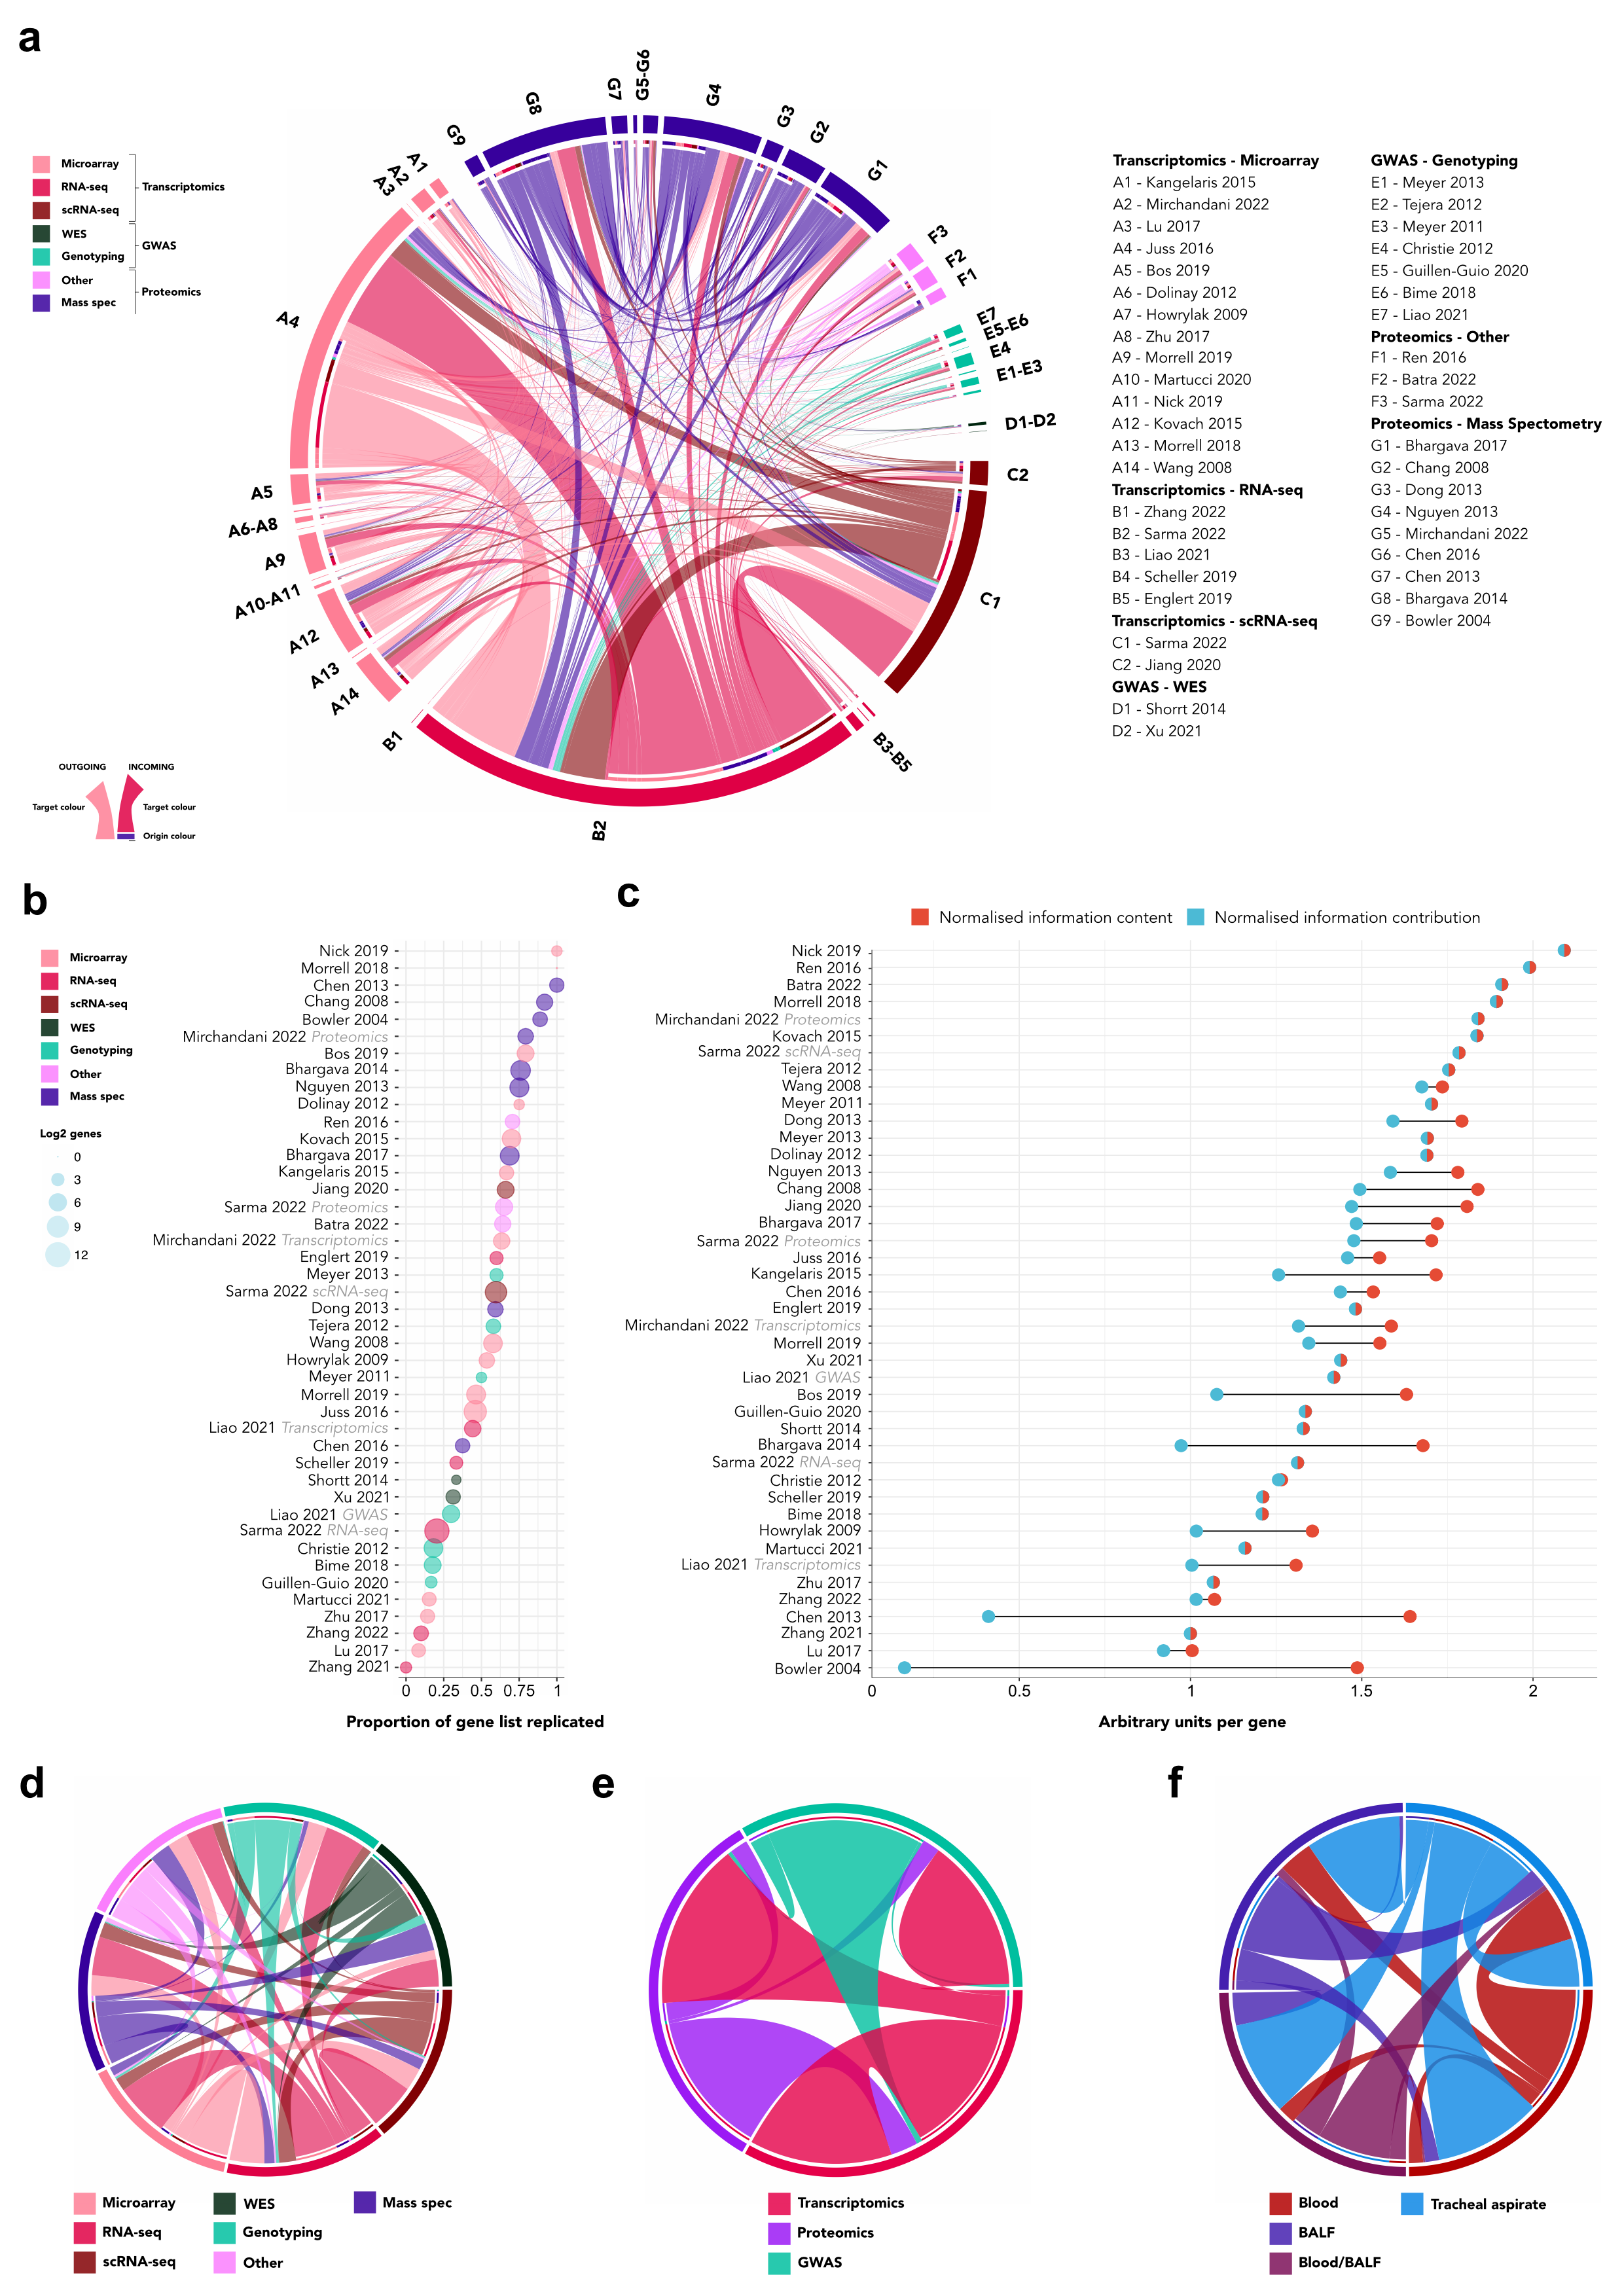
\includegraphics{./img/Figure_2.png}

}

\caption{\label{fig-fig2}\textbf{Functional enrichment of prioritised
genes}. (a) Significantly enriched Reactome terms (\emph{P} \textless{}
0.01). Terms colored by parent class and size proportional to recall.
(b) Euler diagram of the overlap of hub genes identified by five
methods. MNC - Maximum Neighbourhood Component, MCC - Maximal Clique
Centrality, DMNC - Density of MNC, EPC - Edge Percolated Component. (c)
Protein-protein interaction (PPI) network of hub genes, clustered using
the Markov Chain Algorithm. (d). Heatmap of common hub genes displaying
tissue type(s), MAIC score, highest category score, supporting lists,
and presence in the DGIdb druggable genome (indicated in red).}

\end{figure}%

\paragraph{Sub-groups}\label{sub-groups}

A potential limitation of our approach is the disparity in design of
included studies. To address this, we undertook MAIC on subsets of gene
lists, stratified by study focus. There were sufficient lists to make
this tractable for studies focused on ARDS versus non-ARDS controls
(n=28) and studies of ARDS survival and severity (n=7)
(Figure~\ref{fig-fig3}).

For ARDS vs.~non-ARDS controls, there were 15 transcriptomic (54\%), 7
GWAS (25\%), and 6 proteomic lists (21\%). Together, these studies
included 5,713 patients with ARDS. MAIC ranked 2,096 genes
(Figure~\ref{fig-fig3}). The majority of these (n=1,222, 58\%) were
unique to to this sub-group (Figure~\ref{fig-fig3}). Most were
identified in blood, with a small fraction found solely in airways
samples. The inflection point method prioritised the top ranked 130
genes (Fig. S7a). In comparison to the BioLitMine search and the ARDS
Database of Genes, 71/271 and 117/239 genes were found among this set,
respectively (Fig. S7b). A microarray-based transcriptomic list from
Juss \emph{et. al.}\textsuperscript{30} accounted for more than half
(54.7\%) of the relative ICtb, with an additional 12 lists having a
relative ICtb ≥ 1\% (Tab. S4). ORA using Reactome, KEGG, and
WikiPathways identified 25 significantly enriched pathways, including
multiple terms related to cholesterol metabolism and glycolysis
(Figure~\ref{fig-fig4}). A consensus of topological models identified 7
hub genes within a PPI network of prioritised genes. These genes cluster
in a single group, characterised as being related to cholesterol
metabolism (Figure~\ref{fig-fig3}).

For survival, there were 8 gene lists, consisting of 3 transcriptomic
lists (37.5\%), 3 proteomic lists (37.5\%), and 2 GWAS (25\%). Together,
these studies included 644 patients with ARDS. MAIC ranked 463 genes
(Figure~\ref{fig-fig3}). Approximately half of these (n=238, 51\%) were
unique to survival-based lists. In contrast to the ARDS vs.~non-ARDS
analysis, most survival genes were found in airways samples.
Thirty-three genes were prioritised (Fig. S7d). In total, 32/271 of the
BioLitMine ARDS-associated genes and 23/239 of the ARDS Database of
Genes genes were found among the ARDS MAIC survival set (Fig. S7e). The
proteomic and transcriptomic lists from Bhargava
\emph{et.al}\textsuperscript{15} and Morrell \emph{et.
al}\textsuperscript{40} each contributed approximately 30\% of the
relative ICtb (Tab. S5). IL-10 and IL-18 signalling pathways were both
significantly enriched in ORA (Figure~\ref{fig-fig4}). Graph-based
clustering of the prioritised set of survival genes identified a single
large cluster of immune-related genes including, \emph{IL-10},
\emph{CXCL8}, \emph{TNFRSF1A}, and \emph{IL2RA} (Figure~\ref{fig-fig4}).

\begin{figure}

\centering{

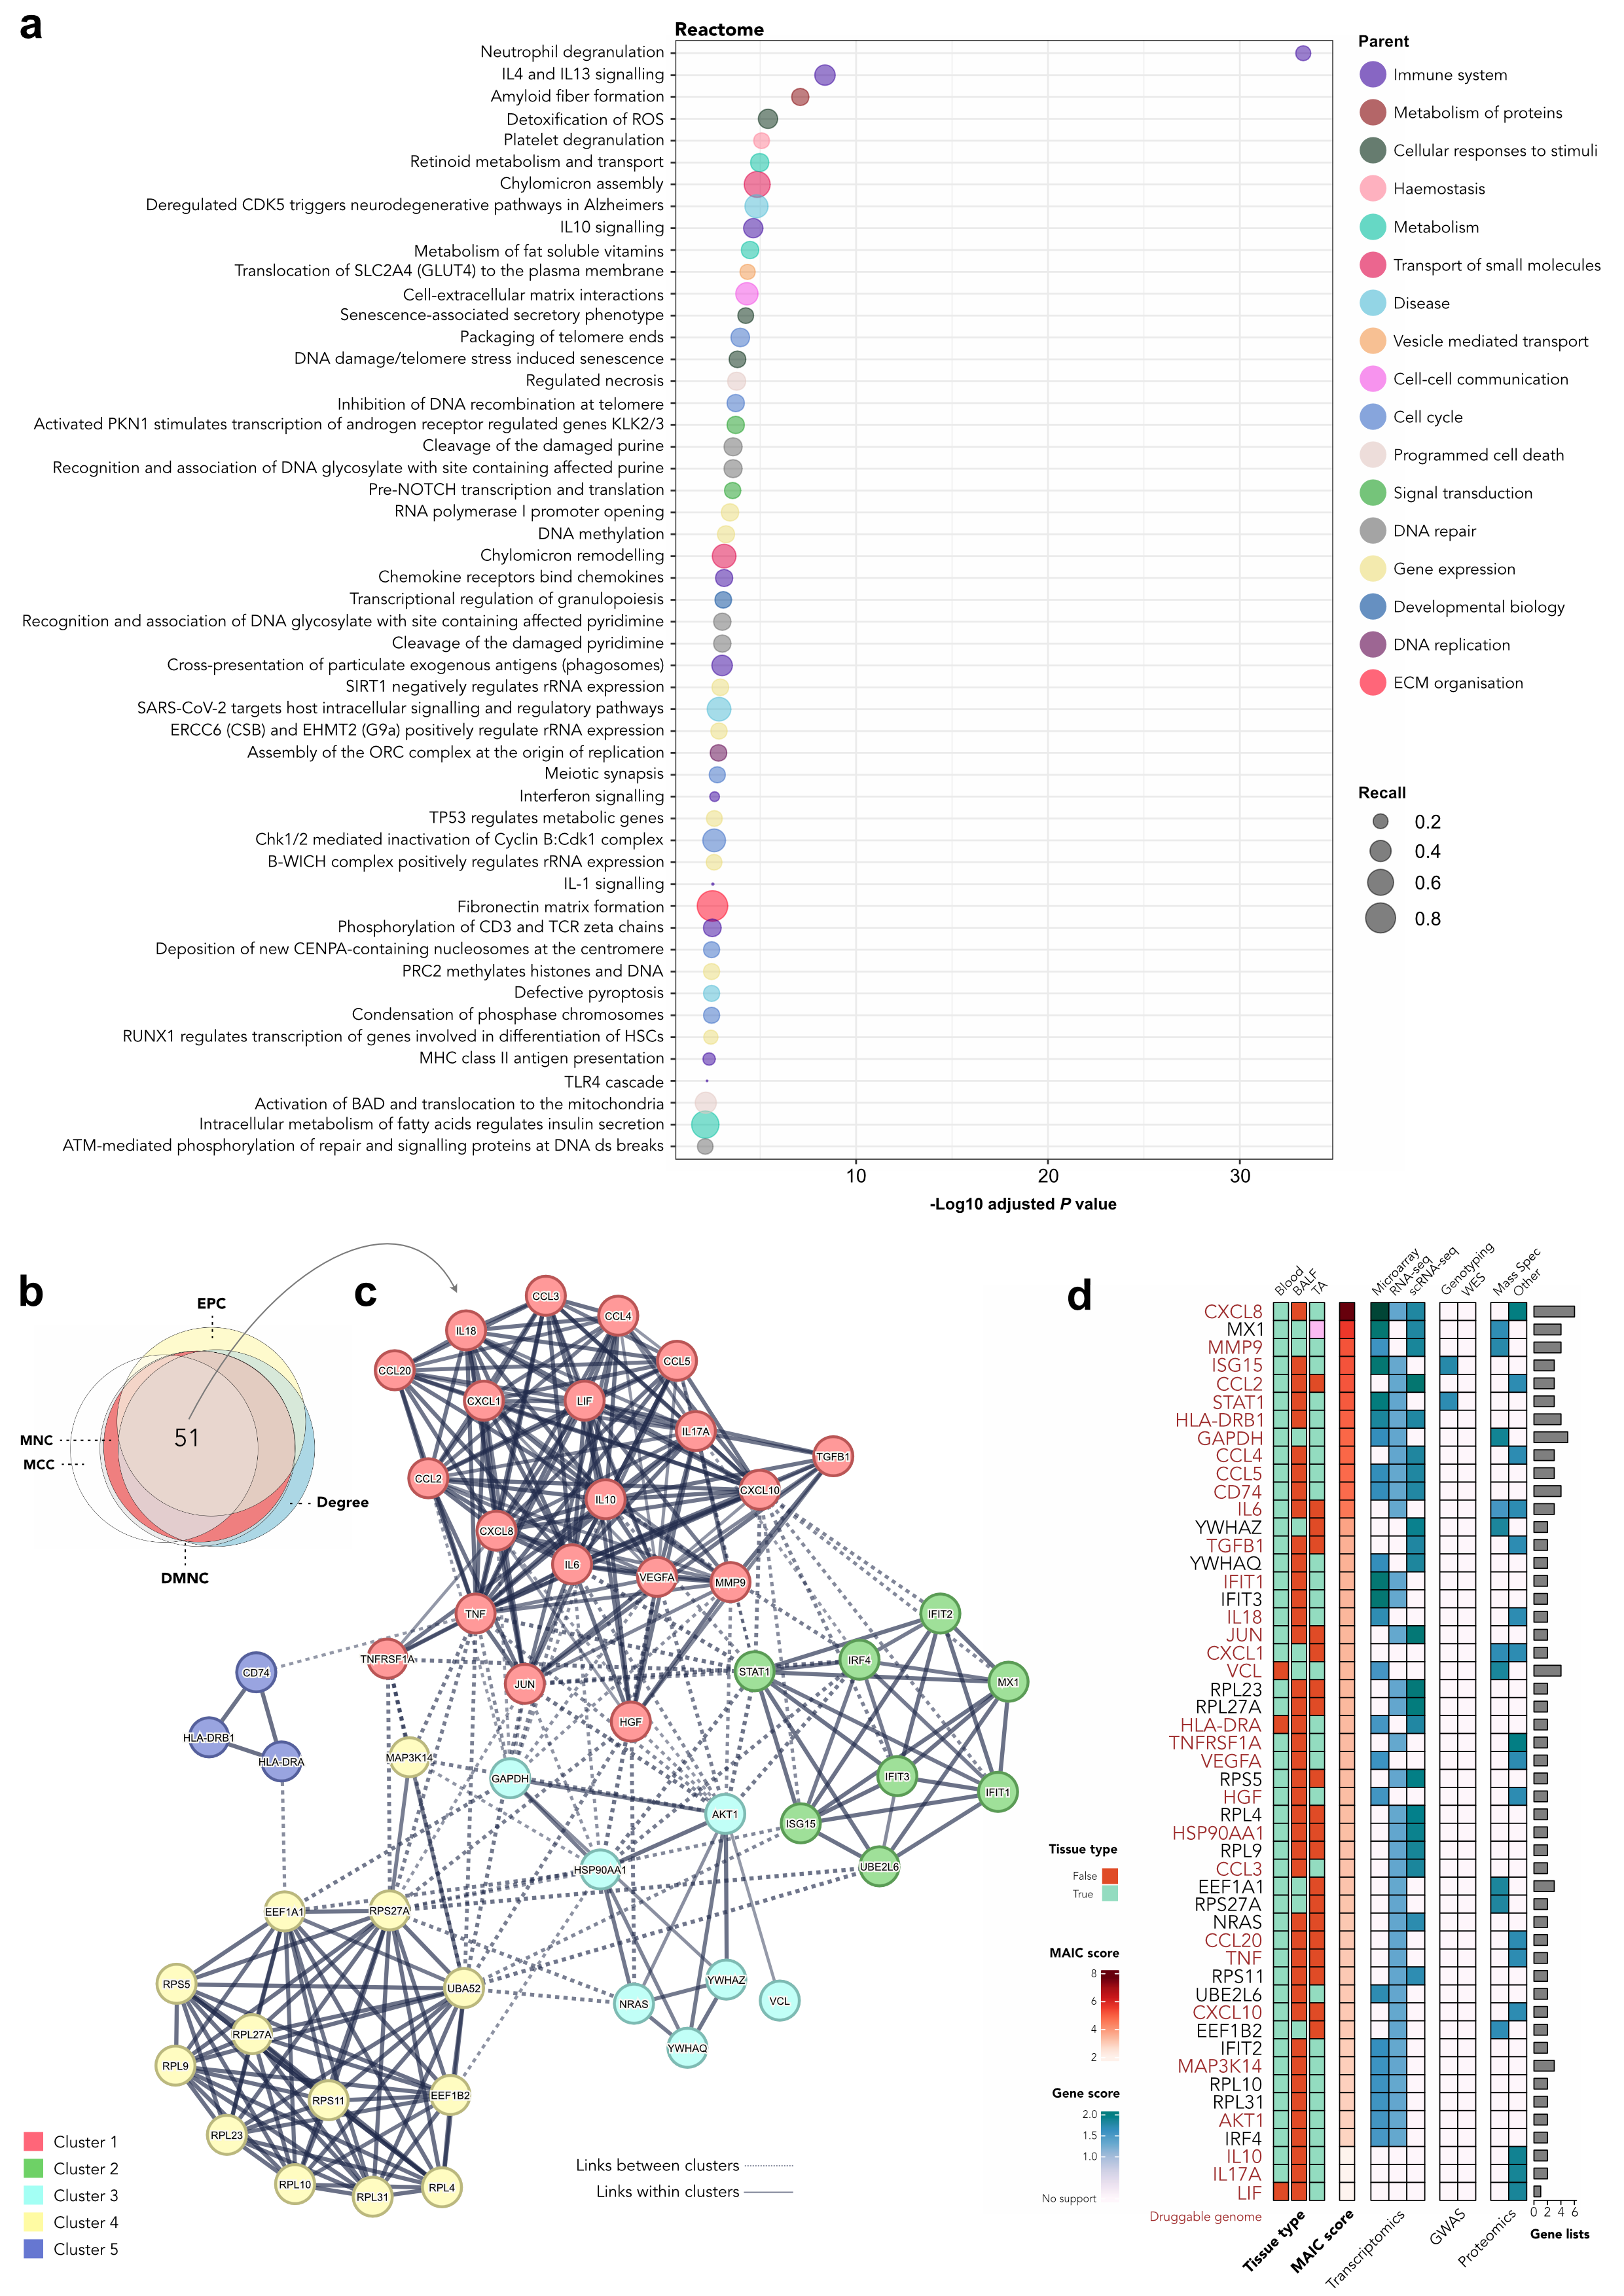
\includegraphics{./img/Figure_3.png}

}

\caption{\label{fig-fig3}\textbf{MAIC of sub-groups}. (a) Schematic of
ARDS MAIC sub-group analyses. (b) Heatmap of top 50 ranked genes in the
ARDS vs.~non-ARDS controls set showing MAIC score, highest score per
category, and number of supporting lists. (c) Heatmap of 16 ranked genes
in the survival set with multi-list support showing MAIC score, highest
score per category, and number of supporting lists. (d) Eular diagram of
gene overlap between the ARDS vs.~non-ARDS controls and survival sets
and the remainder of genes. (e) Bar plots of the tissue type in which
genes are identified. (f) Slope plot comparing the ranks of ARDS
vs.~non-ARDS controls and survival prioritised genes with their ranks in
the full iteration of ARDS MAIC. (g) Euler diagram of the overlap of hub
genes identified by five methods. MNC - Maximum Neighbourhood Component,
MCC - Maximal Clique Centrality, DMNC - Density of MNC, EPC - Edge
Percolated Component and a protein-protein interaction (PPI) network of
hub genes, clustered using the Markov Chain Algorithm - for ARDS
vs.~non-ARDS controls.}

\end{figure}%

\begin{figure}

\centering{

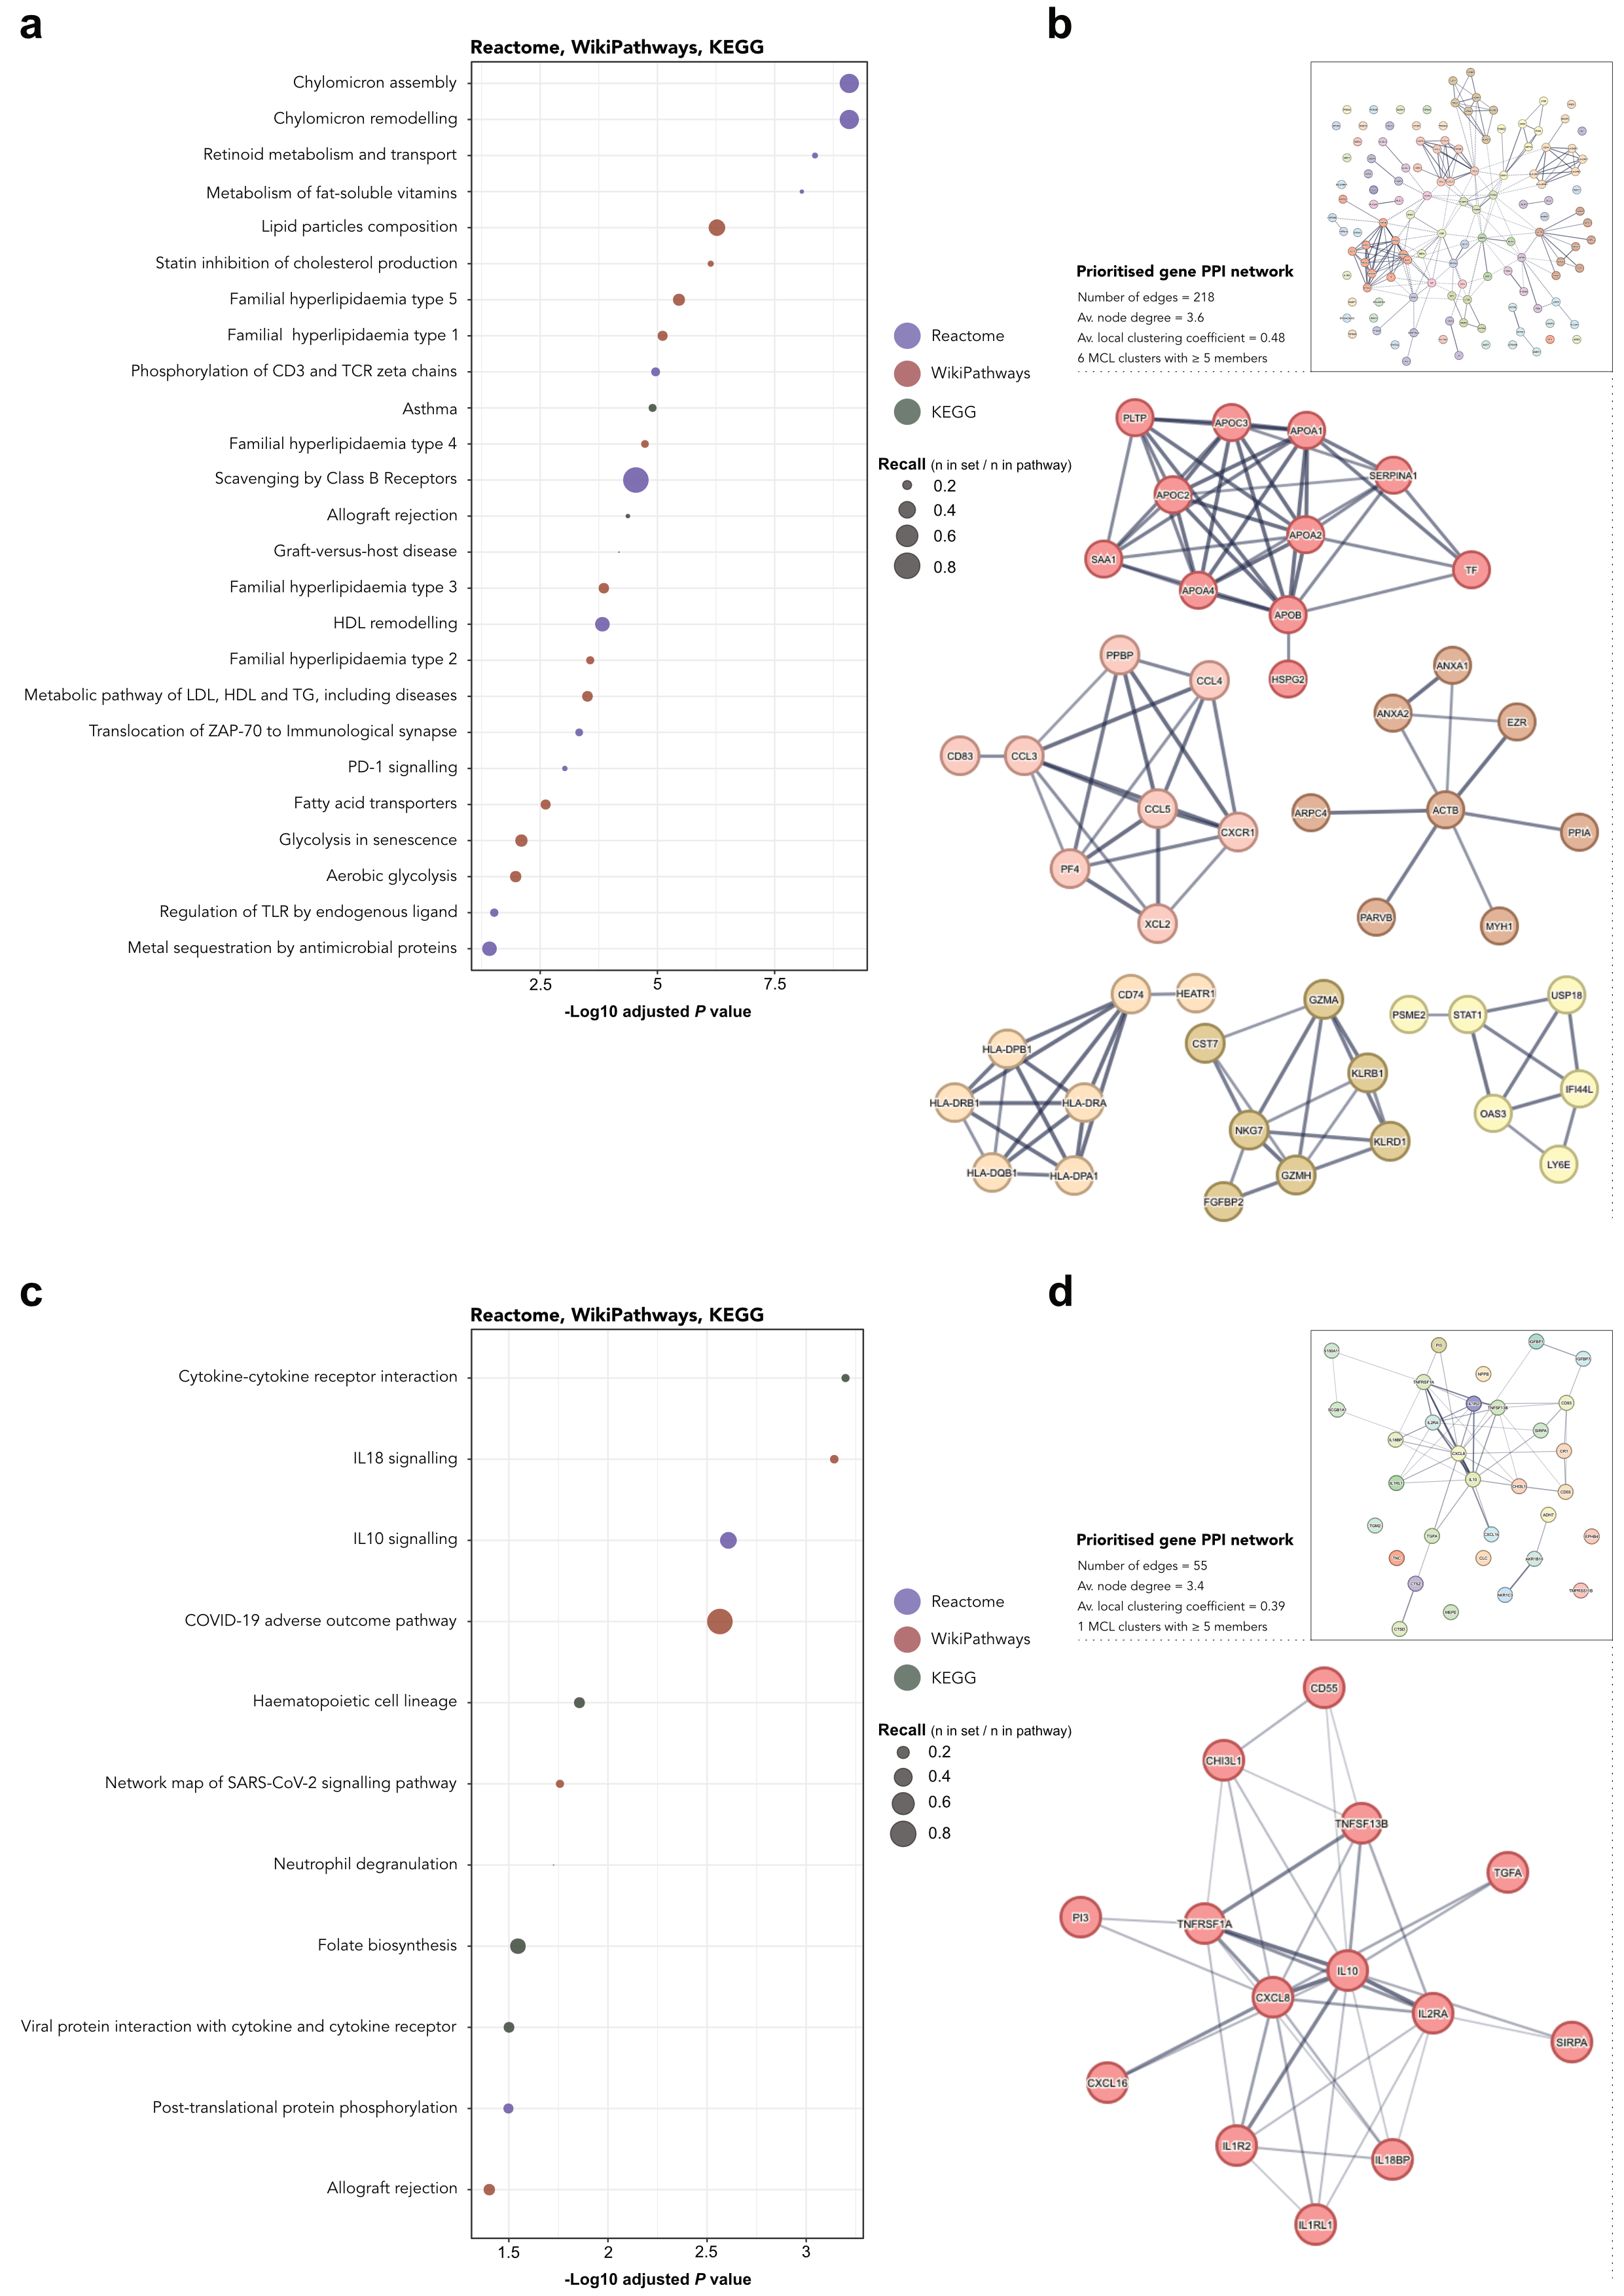
\includegraphics{./img/Figure_4.png}

}

\caption{\label{fig-fig4}\textbf{Sub-group functional enrichment}. (a)
Significantly enriched Reactome, WikiPathways, and KEGG terms (\emph{P}
\textless{} 0.01) for prioritised genes in the ARDS vs.~non-ARDS
controls sub-group. Terms are coloured by pathway and size is
proportional to recall. (b) A protein-protein interaction network of
prioritsed genes in the ARDS vs.~non-ARDS controls cohort and
graph-based clusters with ≥ 5 members. (c) Significantly enriched
Reactome, WikiPathways, and KEGG terms (\emph{P} \textless{} 0.01) for
prioritised genes in the survival sub-group. Terms are coloured by
pathway and size is proportional to recall. (d) A protein-protein
interaction network of prioritsed genes in the survival cohort and
graph-based clusters with ≥ 5 members.}

\end{figure}%

\newpage

\subsection{Discussion}\label{discussion}

Our systematic integration of more than 20 years of data is the first
large-scale meta-analysis of the genomic landscape of ARDS. This
implicates over 7,000 genes and prioritises 1,306. The wide inclusion
criteria capture a diverse range of study designs and methods; the
subsequent application of MAIC establishes the sum of this knowledge,
downgrading noisy, irrelevant, or low-quality information. These results
have three main applications. First, they can be used to better
understand the pathobiology of ARDS, providing a resource to prioritise
future \emph{in-vitro} and \emph{in-vivo} studies and permitting
comparisons between important sub-groups. Second, they prioritise
therapeutic targets, serving as a source against which novel and
repurposed treatments can be screened. Third, they serve as a base for
quantifying the novelty or additive nature of future omics studies in
ARDS.

Our review included 40 studies with genome-wide hypotheses. These
studies varied in their aims and methods, however, some key themes are
of note. Most obviously, the rate at which this form of study is being
published is increasing; half of all studies in the last 5 years and a
quarter since 2020. Similarly, there were few studies which employed
next-generation sequencing (NGS) techniques or equivalent, and only two
single-cell RNA-seq studies. A partial explanation may be the emergence
of COVID-19, which is likely to have consumed the attention of many
research teams active in this field. It is not unreasonable to conclude
that an increasing number of non-COVID ARDS single-cell and NGS studies
will emerge in the coming years. This reinforces the requirement for
methods capable of meta-analysing multi-omic data\textsuperscript{57}.
Less obviously, a minority of studies have sampled the lung in ARDS,
with only four examining the bulk transcriptome in the distal airspace.
Reliance on information derived from blood samples may present a skewed
picture of the pathobiology of ARDS and represents a missed opportunity
to identify novel targets in the lung\textsuperscript{58}.

A key advantage of the MAIC approach is its ability to integrate diverse
data sources. Traditional methods of gene list meta-analysis rely on
simple vote counting or robust rank aggregation\textsuperscript{59}.
Instead, MAIC applies a data-derived weighting to each gene list, allows
the investigator to define granular categorisation (preventing any one
particular method from overwhelming the analysis), and permits the
inclusion of both ranked and unranked lists. We have previously used
MAIC to identify anti-viral genes in response to Influenza A infection,
showing that it outperforms other available methods\textsuperscript{10}.
We have since validated the superiority of MAIC in similar circumstances
in a comprehensive simulation\textsuperscript{12}.

Our prioritisation of genes simultaneously validates existing concepts
of ARDS pathobiology and provides novel insights. The functional
prominence of innate immunity and cytokine signalling - in particular
neutrophil-related activity - is unsurprising\textsuperscript{60}. As is
the high ranking of genes such as \emph{CXCL8}\textsuperscript{61},
\emph{IL-18}\textsuperscript{62}, \emph{MMP9}\textsuperscript{63}, and
\emph{MUC1}\textsuperscript{64}. However, other findings are intriguing.
A single gene example is histidine triad nucleotide binding protein 1
(\emph{HINT1}), ranked 10\textsuperscript{th} and one of only 5 genes to
have support from GWAS, transcriptomics, and proteomics methods. To our
knowledge, no plausible role for \emph{HINT1} has previously been
suggested in ARDS\textsuperscript{65}. However, \emph{HINT1} has been
implicated in T-cell response\textsuperscript{66},
immunoregulation\textsuperscript{67}, and apoptosis\textsuperscript{65}.
Another notable finding is the significant enrichment of cholesterol
uptake, efflux, and esterification pathways among prioritised
genes\textsuperscript{68,69}. Stratification by sub-group offered
further insights. The observation of a tight cluster of genes important
in cholesterol metabolism at the hub of those prioritised in ARDS
vs.~non-ARDS controls is of therapeutic
relevance\textsuperscript{70,71}. However, other programs were observed
in the setting of ARDS vs.~non-ARDS controls including, type I
interferon signalling\textsuperscript{72}, MHC class
II\textsuperscript{73}, cell-cell adhesion\textsuperscript{74}, and
natural killer cell cytotoxicity\textsuperscript{75}. In contrast, genes
prioritised for outcome are functionally more homogeneous and related to
cytokine signalling, in particular IL-10 and IL-18 signalling,
indicating that shared pathways dictate mortality/severity once ARDS is
established.

Our approach has limitations. We purposefully sought studies with
genome-wide hypotheses, excluding single-gene or candidate genetics
studies. In the case of a gene with extensive evidence from the latter,
our methodology may underestimate its association with ARDS. However,
these study designs are subject to other limitations, such as
publication and investigator biases\textsuperscript{76}. In our
iteration of MAIC, we did not account for direction of expression or
effect. For a given gene, if the direction of expression differs between
studies, MAIC may overestimate the strength of evidence associated with
that gene. The inability to account for directionality also limits the
scope of functional enrichment analyses which can be performed.
Similarly, the use of an unsupervised prioritisation threshold may
influence the outcomes of downstream analyses, however principled the
approach. Finally, the general paucity of data, and in particular the
limited number of single-cell transcriptomics (or proteomics) studies,
limits the depth of inference that can be made. It is likely that many
pathological perturbations occur with cell-specificity, which may not be
apparent in bulk analyses of heterogeneous tissues\textsuperscript{77}.
In future. the addition of data from these modalities may reveal
precision targets.

Crucially, we provide an open platform and associated tools to enable
deeper mining of the output. This allows others to re-analyse the data
based on alternative sub-group divisions or to integrate unseen
information. Ongoing multi-omic data integration with this initial study
will further enhance the resolution of the data and increase our
confidence in the results.

In summary, by systematically integrating decades of ARDS genomics, this
study improves the scope for gene prioritisation and enhances molecular
pathophysiological clarity. Our results strongly implicate interferon
signalling and cholesterol metabolism dysregulation, providing a
specific therapeutic targets. Enrichment patterns and sub-group
differences also give clues to genomic drivers of susceptibility,
outcomes, and mortality. This substantially improves our
conceptualisation of the genomic landscape of ARDS, setting the stage
for functional validation.

\newpage

\subsection{Methods}\label{methods}

The systematic review and meta-analysis protocol was registered with the
International Prospective Register of Systematic Reviews (PROSPERO;
CRD42022306270). The review is reported in compliance with the Preferred
Reporting Items for Systematic Reviews and Meta-Analyses (PRISMA)
guidelines\textsuperscript{78}.

\paragraph{Search strategy and selection
criteria}\label{search-strategy-and-selection-criteria}

A detailed description of our search strategy and eligibility criteria
is provided in the Supplementary Methods. Briefly, we searched MEDLINE,
Embase, bioRxiv, medRxiv, the ARDS Database of
Genes\textsuperscript{55}, and the NCBI Gene Expression Omnibus from
inception to April 1\textsuperscript{st}, 2023 without language
restrictions. We also performed single-level backwards and forwards
citation searches using SpiderCite\textsuperscript{79} and hand-searched
recent review articles\textsuperscript{80--83}.

We included human genome-wide studies reporting associations between
genes, transcripts, or proteins and ARDS susceptibility, severity,
survival, or phenotype, accepting any contemporaneous ARDS definition.
We excluded paediatric studies (age \textless{} 18 years), animal
studies, \emph{in-vitro} human ARDS models, candidate \emph{in-vivo} or
\emph{in-vitro studies} (\textless{} 50 genes/proteins), candidate gene
associations, and studies with \textless{} 5 patients per arm (except
scRNA-seq).

\paragraph{Outcomes}\label{outcomes}

We retrieved ranked lists of genes associated with the ARDS host
response, preferring measures of significance and adjusted \emph{P}
values over raw \emph{P} values when multiple ranking measures were
used. We obtained both summary lists (all implicated genes) and
author-defined subgroup lists. To combine subgroup lists into summary
lists, we took the minimum \emph{P} value or maximum effect size. We
excluded genes below the author-defined threshold for
significance/effect magnitude. If unavailable, we excluded genes with
\emph{P} \textgreater{} 0.05, z-score \textless{} 1.96, or log fold
change \textless{} 1.5.

\paragraph{Study selection and data
extraction}\label{study-selection-and-data-extraction}

Article titles and abstracts from our search were stored in Zotero
v6.0-beta (Corporation for Digital Scholarship, United States). Titles
were initially screened by one author using
Screenatron\textsuperscript{79}. Two authors then independently screened
abstracts against eligibility criteria, with a third resolving
inconsistencies. Full texts and supplements of eligible studies were
retrieved and inclusion adjudicated by consensus.

Data were extracted by one author and cross-checked by a second. Gene,
transcript, or protein identifiers were mapped to HGNC symbols or
Ensembl/RefSeq equivalents if no HGNC symbol was available. Unannotated
SNPs were searched in NCBI dbSNP. miRBase (University of Manchester,
United Kingdom) provided miRNA symbols. For microarray probes without
symbols, we used the DAVID Gene Accession Conversion tool (Laboratory of
Human Retrovirology and Immunoinformatics, Frederick National Laboratory
for Cancer Research, United States) to map them to HGNC symbols. We
extracted information relating to study design, methodology, tissue/cell
type, demographics, ARDS aetiology, risk factors, severity, and
outcomes.

\paragraph{Meta-analysis by information content
(MAIC)}\label{meta-analysis-by-information-content-maic-1}

The MAIC algorithm has been described in
detail\textsuperscript{8,10,11,84}. Full documentation and the source
code are available at https://github.com/baillielab/maic. Briefly, MAIC
combines ranked and unranked lists of related named entities, such as
genes, from heterogeneous experimental categories, without prior regard
to the quality of each source. The algorithm makes four key assumptions;
(1) genes associated with ARDS exist as true positives, (2) a gene is
more likely to be a true positive if it is found in more than one
source, (3) the probability of being a true positive is enhanced if the
gene appears in a list that contains a higher proportion of replicated
genes, and (4) the probability is further enhanced if it is found in
more than one category of experiment. Based on these assumptions, MAIC
compares lists with each other, forming a weighting for each source
based on its information content, which is then used to calculate a
score for each gene. The output is a ranked list summarizing the total
information supporting each gene's association with ARDS. We have shown
MAIC outperforms available algorithms, especially with ranked and
unranked heterogeneous data\textsuperscript{84}.

As our primary analysis, we performed MAIC on all summary gene lists,
regardless of study focus. Lists were assigned categories based on their
methodology and experimental technique: genome-wide association study
(GWAS) - genotyping, GWAS - whole exome sequencing, transcriptomics -
microarray, transcriptomics - RNA-sequencing (RNA-seq), transcriptomics
- single cell RNA-seq (scRNA-seq), proteomics - mass spectometry, and
proteomics - other. For secondary analyses, we performed MAIC on subsets
of lists based on study focus (i.e., susceptibility to ARDS or
survival/severity).

In secondary analyses, we repeated this pipeline for gene lists arising
from studies in which the focus was ARDS vs.~non-ARDS controls or ARDS
survival/severity.

For each MAIC iteration, we prioritised genes with sufficient evidential
support for further study (i.e., the gene set before which information
content diminished such that there was little/no corroboration for the
remainder's ARDS association). We used the unit invariant knee
method\textsuperscript{53,85} to identify the elbow point in the
best-fit curve of MAIC scores. Genes with values above this point were
prioritized for downstream analyses.

\paragraph{ARDS literature and SARS-CoV-2
associations}\label{ards-literature-and-sars-cov-2-associations}

We used BioLitMine\textsuperscript{54} to query the NCBI Gene database
for genes associated with the Medical Subject Heading (MeSH) term
``Respiratory Distress Syndrome, Acute'', generating a list of genes and
publications. We descriptively compared the overlap between this list
and the MAIC-ranked gene list. Similar comparisons were made between the
ARDS MAIC results and the gene set in the ARDS Database of
Genes\textsuperscript{55} and a prior MAIC of SARS-CoV-2 host
genomics\textsuperscript{11}.

\paragraph{Tissue expression and
enrichment}\label{tissue-expression-and-enrichment}

Transcript and protein expression data for genes included in ARDS MAIC
were retrieved from the Human Protein Atlas (HPA, version
21.0)\textsuperscript{86}. We investigated mRNA expression in a
consensus scRNA-seq dataset of 81 cells from 31 sources
(\url{https://www.proteinatlas.org/about/assays+annotation\#singlecell_rna})
and in the HPA RNA-seq blood dataset\textsuperscript{87}, containing
expression levels in 18 immune cell types and total peripheral blood
mononuclear cells. To investigate protein expression, we retrieved
tissue-specific expression scores from the HPA\textsuperscript{88}. We
conducted cell-type specific enrichment analysis using
WebCSEA\textsuperscript{89} and extracted the top 20 general cell types
for each query.

\paragraph{Functional enrichment}\label{functional-enrichment-1}

We performed functional enrichment of genes against the universe of all
annotated genes using g:Profiler\textsuperscript{90}. The following data
sources were used; Kyoto Encyclopaedia of Genes and Genomes
(KEGG)\textsuperscript{91}, Reactome\textsuperscript{92},
WikiPathways\textsuperscript{93}, and Gene Ontology\textsuperscript{94}.
Multiple testing was corrected for using the g:SCS
algorithm\textsuperscript{90}, with a threshold of \emph{P} \textless{}
0.01. Input lists were ordered by MAIC score were appropriate. In the
case of GO cellular component terms, we used the REVIGO tool to perform
multi-dimensional scaling of the matrix of all pairwise semantic
similarities\textsuperscript{95}. Enrichment was also performed against
the National Human Genome Research Institute GWAS
Catalog\textsuperscript{96} using the Enrichr
web-interface\textsuperscript{97}. Protein-protein interaction
enrichment was performed using STRING v11\textsuperscript{98}. We
included all possible interaction sources but specified a minimum
interaction score of 0.7. We used the the whole annotated genome as the
statistical background. Markov Clustering Analysis (MCL) was applied to
the resulting network with an inflation parameter of 3. Clusters were
annotated by hand having considered enrichment against KEGG, Reactome,
and WikiPathways. To identify hub genes within the PPI network, we used
cytoHubba\textsuperscript{99} and Cytoscape\textsuperscript{100}. The
highest ranked genes by Maximum Neighbourhood Component (MNC), Maximal
Clique Centrality (MCC), Density of MNC (DMNC), Edge Percolated
Component (EPC), and node degree were retrieved. The intersecting genes
of these methods were deemed hub genes. Hub genes were searched for in
the Drug Gene Interaction Database\textsuperscript{101} to identify if
they were present in the druggable genome. The Drug Gene Interaction
Database (DGIdb) was queried for each ranked gene\textsuperscript{102}.

\paragraph{Software and code
availability}\label{software-and-code-availability}

MAIC is implemented in Python v3.9.7 (Python Software Foundation,
Wilmington, United States). All other analyses were performed with R
v4.2.2 (R Core Team, R Foundation for Statistical Computing, Vienna,
Austria). Code required to reproduce the analyses is available at
\url{https://github.com/JonathanEMillar/ards_maic_analysis}. An R
package (ARDSMAICR) containing the data used in this manuscript and
several functions helpful in analyses is available at
\url{https://github.com/baillielab/ARDSMAICr}.

\newpage

\subsection{References}\label{references}

\phantomsection\label{refs}
\begin{CSLReferences}{0}{0}
\bibitem[\citeproctext]{ref-ARDS_Definition_Task_Force}
\CSLLeftMargin{1. }%
\CSLRightInline{ARDS Definition Task Force \emph{et al.} Acute
respiratory distress syndrome: The berlin definition. \emph{JAMA}
\textbf{307}, 2526--2533 (2012).}

\bibitem[\citeproctext]{ref-Bellani2016}
\CSLLeftMargin{2. }%
\CSLRightInline{Bellani, G. \emph{et al.} Epidemiology, patterns of
care, and mortality for patients with acute respiratory distress
syndrome in intensive care units in 50 countries. \emph{JAMA}
\textbf{315}, 788--800 (2016).}

\bibitem[\citeproctext]{ref-Wilson2020}
\CSLLeftMargin{3. }%
\CSLRightInline{Wilson, J. G. \& Calfee, C. S. {ARDS} subphenotypes:
Understanding a heterogeneous syndrome. \emph{Crit. Care} \textbf{24},
102 (2020).}

\bibitem[\citeproctext]{ref-Laffey2018}
\CSLLeftMargin{4. }%
\CSLRightInline{Laffey, J. G. \& Kavanagh, B. P. Negative trials in
critical care: Why most research is probably wrong. \emph{Lancet Respir.
Med.} \textbf{6}, 659--660 (2018).}

\bibitem[\citeproctext]{ref-Bos2022}
\CSLLeftMargin{5. }%
\CSLRightInline{Bos, L. D. J. \emph{et al.} Towards a biological
definition of {ARDS}: Are treatable traits the solution? \emph{Intensive
Care Med. Exp.} \textbf{10}, 8 (2022).}

\bibitem[\citeproctext]{ref-RECOVERYBari2022}
\CSLLeftMargin{6. }%
\CSLRightInline{Peter W Horby, and \emph{et al.} Baricitinib in patients
admitted to hospital with {COVID}-19 ({RECOVERY}): A randomised,
controlled, open-label, platform trial and updated meta-analysis. (2022)
doi:\href{https://doi.org/10.1101/2022.03.02.22271623}{10.1101/2022.03.02.22271623}.}

\bibitem[\citeproctext]{ref-pmid32032529}
\CSLLeftMargin{7. }%
\CSLRightInline{Richardson, P. \emph{et al.} {{B}aricitinib as potential
treatment for 2019-n{C}o{V} acute respiratory disease}. \emph{Lancet}
\textbf{395}, e30--e31 (2020).}

\bibitem[\citeproctext]{ref-Pairo-Castineira2021}
\CSLLeftMargin{8. }%
\CSLRightInline{Pairo-Castineira, E. \emph{et al.} Genetic mechanisms of
critical illness in {COVID-19}. \emph{Nature} \textbf{591}, 92--98
(2021).}

\bibitem[\citeproctext]{ref-Gomez-Cabrero2014}
\CSLLeftMargin{9. }%
\CSLRightInline{Gomez-Cabrero, D. \emph{et al.} Data integration in the
era of omics: Current and future challenges. \emph{BMC Syst. Biol.}
\textbf{8 Suppl 2}, I1 (2014).}

\bibitem[\citeproctext]{ref-Li2020}
\CSLLeftMargin{10. }%
\CSLRightInline{Li, B. \emph{et al.} Genome-wide {CRISPR} screen
identifies host dependency factors for influenza a virus infection.
\emph{Nat. Commun.} \textbf{11}, 164 (2020).}

\bibitem[\citeproctext]{ref-Parkinson2020}
\CSLLeftMargin{11. }%
\CSLRightInline{Parkinson, N. \emph{et al.} Dynamic data-driven
meta-analysis for prioritisation of host genes implicated in {COVID-19}.
\emph{Sci. Rep.} \textbf{10}, 22303 (2020).}

\bibitem[\citeproctext]{ref-pmid36094347}
\CSLLeftMargin{12. }%
\CSLRightInline{Wang, B. \emph{et al.} {{S}ystematic comparison of
ranking aggregation methods for gene lists in experimental results}.
\emph{Bioinformatics} \textbf{38}, 4927--4933 (2022).}

\bibitem[\citeproctext]{ref-Batra2022}
\CSLLeftMargin{13. }%
\CSLRightInline{Batra, R. \emph{et al.} Multi-omic comparative analysis
of {COVID-19} and bacterial sepsis-induced {ARDS}. \emph{PLoS Pathog.}
\textbf{18}, e1010819 (2022).}

\bibitem[\citeproctext]{ref-Bhargava2014}
\CSLLeftMargin{14. }%
\CSLRightInline{Bhargava, M. \emph{et al.} Proteomic profiles in acute
respiratory distress syndrome differentiates survivors from
non-survivors. \emph{PLoS One} \textbf{9}, e109713 (2014).}

\bibitem[\citeproctext]{ref-Bhargava2017}
\CSLLeftMargin{15. }%
\CSLRightInline{Bhargava, M. \emph{et al.} Bronchoalveolar lavage fluid
protein expression in acute respiratory distress syndrome provides
insights into pathways activated in subjects with different outcomes.
\emph{Sci. Rep.} \textbf{7}, 7464 (2017).}

\bibitem[\citeproctext]{ref-Bime2018}
\CSLLeftMargin{16. }%
\CSLRightInline{Bime, C. \emph{et al.} Genome-wide association study in
african americans with acute respiratory distress syndrome identifies
the selectin {P} ligand gene as a risk factor. \emph{Am. J. Respir.
Crit. Care Med.} \textbf{197}, 1421--1432 (2018).}

\bibitem[\citeproctext]{ref-Bos2019}
\CSLLeftMargin{17. }%
\CSLRightInline{Bos, L. D. J. \emph{et al.} Understanding heterogeneity
in biologic phenotypes of acute respiratory distress syndrome by
leukocyte expression profiles. \emph{Am. J. Respir. Crit. Care Med.}
\textbf{200}, 42--50 (2019).}

\bibitem[\citeproctext]{ref-Bowler2004}
\CSLLeftMargin{18. }%
\CSLRightInline{Bowler, R. P. \emph{et al.} Proteomic analysis of
pulmonary edema fluid and plasma in patients with acute lung injury.
\emph{Am. J. Physiol. Lung Cell. Mol. Physiol.} \textbf{286}, L1095--104
(2004).}

\bibitem[\citeproctext]{ref-Chang2008}
\CSLLeftMargin{19. }%
\CSLRightInline{Chang, D. W. \emph{et al.} Proteomic and computational
analysis of bronchoalveolar proteins during the course of the acute
respiratory distress syndrome. \emph{Am. J. Respir. Crit. Care Med.}
\textbf{178}, 701--709 (2008).}

\bibitem[\citeproctext]{ref-Chen2013}
\CSLLeftMargin{20. }%
\CSLRightInline{Chen, X., Shan, Q., Jiang, L., Zhu, B. \& Xi, X.
Quantitative proteomic analysis by {iTRAQ} for identification of
candidate biomarkers in plasma from acute respiratory distress syndrome
patients. \emph{Biochem. Biophys. Res. Commun.} \textbf{441}, 1--6
(2013).}

\bibitem[\citeproctext]{ref-Chen2016}
\CSLLeftMargin{21. }%
\CSLRightInline{Chen, C., Shi, L., Li, Y., Wang, X. \& Yang, S.
Disease-specific dynamic biomarkers selected by integrating inflammatory
mediators with clinical informatics in {ARDS} patients with severe
pneumonia. \emph{Cell Biol. Toxicol.} \textbf{32}, 169--184 (2016).}

\bibitem[\citeproctext]{ref-Christie2012}
\CSLLeftMargin{22. }%
\CSLRightInline{Christie, J. D. \emph{et al.} Genome wide association
identifies {PPFIA1} as a candidate gene for acute lung injury risk
following major trauma. \emph{PLoS One} \textbf{7}, e28268 (2012).}

\bibitem[\citeproctext]{ref-Dolinay2012}
\CSLLeftMargin{23. }%
\CSLRightInline{Dolinay, T. \emph{et al.} Inflammasome-regulated
cytokines are critical mediators of acute lung injury. \emph{Am. J.
Respir. Crit. Care Med.} \textbf{185}, 1225--1234 (2012).}

\bibitem[\citeproctext]{ref-Dong2013}
\CSLLeftMargin{24. }%
\CSLRightInline{Dong, H. \emph{et al.} Comparative analysis of the
alveolar macrophage proteome in {ALI/ARDS} patients between the
exudative phase and recovery phase. \emph{BMC Immunol.} \textbf{14}, 25
(2013).}

\bibitem[\citeproctext]{ref-Englert2019}
\CSLLeftMargin{25. }%
\CSLRightInline{Englert, J. A. \emph{et al.} Whole blood {RNA}
sequencing reveals a unique transcriptomic profile in patients with
{ARDS} following hematopoietic stem cell transplantation. \emph{Respir.
Res.} \textbf{20}, 15 (2019).}

\bibitem[\citeproctext]{ref-Frenzel2011}
\CSLLeftMargin{26. }%
\CSLRightInline{Frenzel, J. \emph{et al.} Outcome prediction in
pneumonia induced {ALI/ARDS} by clinical features and peptide patterns
of {BALF} determined by mass spectrometry. \emph{PLoS One} \textbf{6},
e25544 (2011).}

\bibitem[\citeproctext]{ref-GuillenGuio2020}
\CSLLeftMargin{27. }%
\CSLRightInline{Guillen-Guio, B. \emph{et al.} Sepsis-associated acute
respiratory distress syndrome in individuals of european ancestry: A
genome-wide association study. \emph{Lancet Respir. Med.} \textbf{8},
258--266 (2020).}

\bibitem[\citeproctext]{ref-Howrylak2009}
\CSLLeftMargin{28. }%
\CSLRightInline{Howrylak, J. A. \emph{et al.} Discovery of the gene
signature for acute lung injury in patients with sepsis. \emph{Physiol.
Genomics} \textbf{37}, 133--139 (2009).}

\bibitem[\citeproctext]{ref-Jiang2020}
\CSLLeftMargin{29. }%
\CSLRightInline{Jiang, Y. \emph{et al.} Single cell {RNA} sequencing
identifies an early monocyte gene signature in acute respiratory
distress syndrome. \emph{JCI Insight} \textbf{5}, (2020).}

\bibitem[\citeproctext]{ref-Juss2016}
\CSLLeftMargin{30. }%
\CSLRightInline{Juss, J. K. \emph{et al.} Acute respiratory distress
syndrome neutrophils have a distinct phenotype and are resistant to
phosphoinositide 3-kinase inhibition. \emph{Am. J. Respir. Crit. Care
Med.} \textbf{194}, 961--973 (2016).}

\bibitem[\citeproctext]{ref-Kangelaris2015}
\CSLLeftMargin{31. }%
\CSLRightInline{Kangelaris, K. N. \emph{et al.} Increased expression of
neutrophil-related genes in patients with early sepsis-induced {ARDS}.
\emph{Am. J. Physiol. Lung Cell. Mol. Physiol.} \textbf{308}, L1102--13
(2015).}

\bibitem[\citeproctext]{ref-Kovach2015}
\CSLLeftMargin{32. }%
\CSLRightInline{Kovach, M. A. \emph{et al.} Microarray analysis
identifies {IL-1} receptor type 2 as a novel candidate biomarker in
patients with acute respiratory distress syndrome. \emph{Respir. Res.}
\textbf{16}, 29 (2015).}

\bibitem[\citeproctext]{ref-Liao2021}
\CSLLeftMargin{33. }%
\CSLRightInline{Liao, S. Y. \emph{et al.} Identification of early and
intermediate biomarkers for {ARDS} mortality by multi-omic approaches.
\emph{Sci. Rep.} \textbf{11}, 18874 (2021).}

\bibitem[\citeproctext]{ref-Lu2017}
\CSLLeftMargin{34. }%
\CSLRightInline{Lu, X.-G. \emph{et al.} Circulating {miRNAs} as
biomarkers for severe acute pancreatitis associated with acute lung
injury. \emph{World J. Gastroenterol.} \textbf{23}, 7440--7449 (2017).}

\bibitem[\citeproctext]{ref-Martucci2020}
\CSLLeftMargin{35. }%
\CSLRightInline{Martucci, G. \emph{et al.} Identification of a
circulating {miRNA} signature to stratify acute respiratory distress
syndrome patients. \emph{J. Pers. Med.} \textbf{11}, 15 (2020).}

\bibitem[\citeproctext]{ref-Meyer2011}
\CSLLeftMargin{36. }%
\CSLRightInline{Meyer, N. J. \emph{et al.} {ANGPT2} genetic variant is
associated with trauma-associated acute lung injury and altered plasma
angiopoietin-2 isoform ratio. \emph{Am. J. Respir. Crit. Care Med.}
\textbf{183}, 1344--1353 (2011).}

\bibitem[\citeproctext]{ref-Meyer2013}
\CSLLeftMargin{37. }%
\CSLRightInline{Meyer, N. J. \emph{et al.} {IL1RN} coding variant is
associated with lower risk of acute respiratory distress syndrome and
increased plasma {IL-1} receptor antagonist. \emph{Am. J. Respir. Crit.
Care Med.} \textbf{187}, 950--959 (2013).}

\bibitem[\citeproctext]{ref-Mirchandani2022}
\CSLLeftMargin{38. }%
\CSLRightInline{Mirchandani, A. S. \emph{et al.} Hypoxia shapes the
immune landscape in lung injury and promotes the persistence of
inflammation. \emph{Nat. Immunol.} \textbf{23}, 927--939 (2022).}

\bibitem[\citeproctext]{ref-Morrell2018}
\CSLLeftMargin{39. }%
\CSLRightInline{Morrell, E. D. \emph{et al.} Cytometry {TOF} identifies
alveolar macrophage subtypes in acute respiratory distress syndrome.
\emph{JCI Insight} \textbf{3}, (2018).}

\bibitem[\citeproctext]{ref-Morrell2019}
\CSLLeftMargin{40. }%
\CSLRightInline{Morrell, E. D. \emph{et al.} Alveolar macrophage
transcriptional programs are associated with outcomes in acute
respiratory distress syndrome. \emph{Am. J. Respir. Crit. Care Med.}
\textbf{200}, 732--741 (2019).}

\bibitem[\citeproctext]{ref-Nick2016}
\CSLLeftMargin{41. }%
\CSLRightInline{Nick, J. A. \emph{et al.} Extremes of
interferon-stimulated gene expression associate with worse outcomes in
the acute respiratory distress syndrome. \emph{PLoS One} \textbf{11},
e0162490 (2016).}

\bibitem[\citeproctext]{ref-Nguyen2013}
\CSLLeftMargin{42. }%
\CSLRightInline{Nguyen, E. V. \emph{et al.} Proteomic profiling of
bronchoalveolar lavage fluid in critically ill patients with
ventilator-associated pneumonia. \emph{PLoS One} \textbf{8}, e58782
(2013).}

\bibitem[\citeproctext]{ref-Ren2016}
\CSLLeftMargin{43. }%
\CSLRightInline{Ren, S. \emph{et al.} Deleted in malignant brain tumors
1 protein is a potential biomarker of acute respiratory distress
syndrome induced by pneumonia. \emph{Biochem. Biophys. Res. Commun.}
\textbf{478}, 1344--1349 (2016).}

\bibitem[\citeproctext]{ref-Sarma2022}
\CSLLeftMargin{44. }%
\CSLRightInline{Sarma, A. \emph{et al.} Hyperinflammatory {ARDS} is
characterized by interferon-stimulated gene expression, t-cell
activation, and an altered metatranscriptome in tracheal aspirates.
\emph{bioRxiv} (2022).}

\bibitem[\citeproctext]{ref-Scheller2019}
\CSLLeftMargin{45. }%
\CSLRightInline{Scheller, N. \emph{et al.} Proviral {MicroRNAs} detected
in extracellular vesicles from bronchoalveolar lavage fluid of patients
with influenza virus-induced acute respiratory distress syndrome.
\emph{J. Infect. Dis.} \textbf{219}, 540--543 (2019).}

\bibitem[\citeproctext]{ref-Shortt2014}
\CSLLeftMargin{46. }%
\CSLRightInline{Shortt, K. \emph{et al.} Identification of novel single
nucleotide polymorphisms associated with acute respiratory distress
syndrome by exome-seq. \emph{PLoS One} \textbf{9}, e111953 (2014).}

\bibitem[\citeproctext]{ref-Wang2008}
\CSLLeftMargin{47. }%
\CSLRightInline{Wang, Z., Beach, D., Su, L., Zhai, R. \& Christiani, D.
C. A genome-wide expression analysis in blood identifies pre-elafin as a
biomarker in {ARDS}. \emph{Am. J. Respir. Cell Mol. Biol.} \textbf{38},
724--732 (2008).}

\bibitem[\citeproctext]{ref-Tejera2012}
\CSLLeftMargin{48. }%
\CSLRightInline{Tejera, P. \emph{et al.} Distinct and replicable genetic
risk factors for acute respiratory distress syndrome of pulmonary or
extrapulmonary origin. \emph{J. Med. Genet.} \textbf{49}, 671--680
(2012).}

\bibitem[\citeproctext]{ref-Xu2021}
\CSLLeftMargin{49. }%
\CSLRightInline{Xu, J.-Y. \emph{et al.} Nucleotide polymorphism in
{ARDS} outcome: A whole exome sequencing association study. \emph{Ann.
Transl. Med.} \textbf{9}, 780 (2021).}

\bibitem[\citeproctext]{ref-Zhang2021}
\CSLLeftMargin{50. }%
\CSLRightInline{Zhang, S. \emph{et al.} miR-584 and miR-146 are
candidate biomarkers for acute respiratory distress syndrome. \emph{Exp.
Ther. Med.} \textbf{21}, 445 (2021).}

\bibitem[\citeproctext]{ref-Zhang2022}
\CSLLeftMargin{51. }%
\CSLRightInline{Zhang, C. \emph{et al.} Differential expression profile
of plasma exosomal {microRNAs} in acute type a aortic dissection with
acute lung injury. \emph{Sci. Rep.} \textbf{12}, 11667 (2022).}

\bibitem[\citeproctext]{ref-Zhu2017}
\CSLLeftMargin{52. }%
\CSLRightInline{Zhu, Z. \emph{et al.} Whole blood {microRNA} markers are
associated with acute respiratory distress syndrome. \emph{Intensive
Care Med. Exp.} \textbf{5}, 38 (2017).}

\bibitem[\citeproctext]{ref-Christopoulos2016-jb}
\CSLLeftMargin{53. }%
\CSLRightInline{Christopoulos, D. Introducing unit invariant knee
({UIK}) as an objective choice for elbow point in multivariate data
analysis techniques. \emph{SSRN Electron. J.} (2016).}

\bibitem[\citeproctext]{ref-Hu2020-dl}
\CSLLeftMargin{54. }%
\CSLRightInline{Hu, Y. \emph{et al.} {BioLitMine}: Advanced mining of
biomedical and biological literature about human genes and genes from
major model organisms. \emph{G3 (Bethesda)} \textbf{10}, 4531--4539
(2020).}

\bibitem[\citeproctext]{ref-Quintanilla2021}
\CSLLeftMargin{55. }%
\CSLRightInline{Quintanilla, E., Diwa, K., Nguyen, A., Vu, L. \& Toby,
I. T. A data report on the curation and development of a database of
genes for acute respiratory distress syndrome. \emph{Front. Genet.}
\textbf{12}, 750568 (2021).}

\bibitem[\citeproctext]{ref-Lachmann2018}
\CSLLeftMargin{56. }%
\CSLRightInline{Lachmann, A. \emph{et al.} Massive mining of publicly
available {RNA-seq} data from human and mouse. \emph{Nat. Commun.}
\textbf{9}, 1366 (2018).}

\bibitem[\citeproctext]{ref-pmid35817619}
\CSLLeftMargin{57. }%
\CSLRightInline{Fischer, M. \& Hoffmann, S. {{S}ynthesizing genome
regulation data with vote-counting}. \emph{Trends Genet} \textbf{38},
1208--1216 (2022).}

\bibitem[\citeproctext]{ref-pmid35274164}
\CSLLeftMargin{58. }%
\CSLRightInline{Bos, L. D. J. \emph{et al.} {{T}owards a biological
definition of {A}{R}{D}{S}: are treatable traits the solution?}
\emph{Intensive Care Med Exp} \textbf{10}, 8 (2022).}

\bibitem[\citeproctext]{ref-pmid22247279}
\CSLLeftMargin{59. }%
\CSLRightInline{Kolde, R., Laur, S., Adler, P. \& Vilo, J. {{R}obust
rank aggregation for gene list integration and meta-analysis}.
\emph{Bioinformatics} \textbf{28}, 573--580 (2012).}

\bibitem[\citeproctext]{ref-pmid921049}
\CSLLeftMargin{60. }%
\CSLRightInline{Bachofen, M. \& Weibel, E. R. {{A}lterations of the gas
exchange apparatus in adult respiratory insufficiency associated with
septicemia}. \emph{Am Rev Respir Dis} \textbf{116}, 589--615 (1977).}

\bibitem[\citeproctext]{ref-pmid36725964}
\CSLLeftMargin{61. }%
\CSLRightInline{Cambier, S., Gouwy, M. \& Proost, P. {{T}he chemokines
{C}{X}{C}{L}8 and {C}{X}{C}{L}12: molecular and functional properties,
role in disease and efforts towards pharmacological intervention}.
\emph{Cell Mol Immunol} \textbf{20}, 217--251 (2023).}

\bibitem[\citeproctext]{ref-pmid37695136}
\CSLLeftMargin{62. }%
\CSLRightInline{Moore, A. R. \emph{et al.} {{E}levated {P}lasma
{I}nterleukin-18 {I}dentifies {H}igh-{R}isk {A}cute {R}espiratory
{D}istress {S}yndrome {P}atients not {D}istinguished by {P}rior {L}atent
{C}lass {A}nalyses {U}sing {T}raditional {I}nflammatory {C}ytokines: {A}
{R}etrospective {A}nalysis of {T}wo {R}andomized {C}linical {T}rials}.
\emph{Crit Care Med} (2023).}

\bibitem[\citeproctext]{ref-pmid21565917}
\CSLLeftMargin{63. }%
\CSLRightInline{Davey, A., McAuley, D. F. \& O'Kane, C. M. {{M}atrix
metalloproteinases in acute lung injury: mediators of injury and drivers
of repair}. \emph{Eur Respir J} \textbf{38}, 959--970 (2011).}

\bibitem[\citeproctext]{ref-pmid33536260}
\CSLLeftMargin{64. }%
\CSLRightInline{Ballester, B., Milara, J. \& Cortijo, J. {{T}he role of
mucin 1 in respiratory diseases}. \emph{Eur Respir Rev} \textbf{30},
(2021).}

\bibitem[\citeproctext]{ref-pmid16835243}
\CSLLeftMargin{65. }%
\CSLRightInline{Weiske, J. \& Huber, O. {{T}he histidine triad protein
{H}int1 triggers apoptosis independent of its enzymatic activity}.
\emph{J Biol Chem} \textbf{281}, 27356--27366 (2006).}

\bibitem[\citeproctext]{ref-pmid36846002}
\CSLLeftMargin{66. }%
\CSLRightInline{Wang, X., Zhou, M. \& Jiang, L. {{T}he oncogenic and
immunological roles of histidine triad nucleotide-binding protein 1 in
human cancers and their experimental validation in the {M}{C}{F}-7 cell
line}. \emph{Ann Transl Med} \textbf{11}, 147 (2023).}

\bibitem[\citeproctext]{ref-pmid25092109}
\CSLLeftMargin{67. }%
\CSLRightInline{Galazka, G. \emph{et al.} {{H}{I}{N}{T}1 peptide/{H}sp70
complex induces {N}{K}-cell-dependent immunoregulation in a model of
autoimmune demyelination}. \emph{Eur J Immunol} \textbf{44}, 3026--3044
(2014).}

\bibitem[\citeproctext]{ref-pmid22706330}
\CSLLeftMargin{68. }%
\CSLRightInline{Gowdy, K. M. \& Fessler, M. B. {{E}merging roles for
cholesterol and lipoproteins in lung disease}. \emph{Pulm Pharmacol
Ther} \textbf{26}, 430--437 (2013).}

\bibitem[\citeproctext]{ref-pmid34715007}
\CSLLeftMargin{69. }%
\CSLRightInline{Hofmaenner, D. A., Kleyman, A., Press, A., Bauer, M. \&
Singer, M. {{T}he {M}any {R}oles of {C}holesterol in {S}epsis: {A}
{R}eview}. \emph{Am J Respir Crit Care Med} \textbf{205}, 388--396
(2022).}

\bibitem[\citeproctext]{ref-pmid36978134}
\CSLLeftMargin{70. }%
\CSLRightInline{Pienkos, S. M. \emph{et al.} {{E}ffect of total
cholesterol and statin therapy on mortality in {A}{R}{D}{S} patients: a
secondary analysis of the {S}{A}{I}{L}{S} and {H}{A}{R}{P}-2 trials}.
\emph{Crit Care} \textbf{27}, 126 (2023).}

\bibitem[\citeproctext]{ref-pmid35770004}
\CSLLeftMargin{71. }%
\CSLRightInline{Metkus, T. S. \emph{et al.} {{P}lasma {P}roprotein
{C}onvertase {S}ubtilisin/kexin {T}ype 9 ({P}{C}{S}{K}9) in the {A}cute
{R}espiratory {D}istress {S}yndrome}. \emph{Front Med (Lausanne)}
\textbf{9}, 876046 (2022).}

\bibitem[\citeproctext]{ref-pmid32661059}
\CSLLeftMargin{72. }%
\CSLRightInline{Hadjadj, J. \emph{et al.} {{I}mpaired type {I}
interferon activity and inflammatory responses in severe
{C}{O}{V}{I}{D}-19 patients}. \emph{Science} \textbf{369}, 718--724
(2020).}

\bibitem[\citeproctext]{ref-pmid28449694}
\CSLLeftMargin{73. }%
\CSLRightInline{Matzaraki, V., Kumar, V., Wijmenga, C. \& Zhernakova, A.
{{T}he {M}{H}{C} locus and genetic susceptibility to autoimmune and
infectious diseases}. \emph{Genome Biol} \textbf{18}, 76 (2017).}

\bibitem[\citeproctext]{ref-pmid12237888}
\CSLLeftMargin{74. }%
\CSLRightInline{ller, A. M., Cronen, C., ller, K. M. \& Kirkpatrick, C.
J. {{H}eterogeneous expression of cell adhesion molecules by endothelial
cells in {A}{R}{D}{S}}. \emph{J Pathol} \textbf{198}, 270--275 (2002).}

\bibitem[\citeproctext]{ref-pmid32612152}
\CSLLeftMargin{75. }%
\CSLRightInline{Demaria, O. \emph{et al.} {{I}dentification of druggable
inhibitory immune checkpoints on {N}atural {K}iller cells in
{C}{O}{V}{I}{D}-19}. \emph{Cell Mol Immunol} \textbf{17}, 995--997
(2020).}

\bibitem[\citeproctext]{ref-pmid34309672}
\CSLLeftMargin{76. }%
\CSLRightInline{Menon, D. K. \& Rosand, J. {{F}inding a {P}lace for
{C}andidate {G}ene {S}tudies in a {G}enome-{W}ide {A}ssociation {S}tudy
{W}orld}. \emph{JAMA Netw Open} \textbf{4}, e2118594 (2021).}

\bibitem[\citeproctext]{ref-pmid34446707}
\CSLLeftMargin{77. }%
\CSLRightInline{Sarma, A. \emph{et al.} {{T}racheal aspirate {R}{N}{A}
sequencing identifies distinct immunological features of
{C}{O}{V}{I}{D}-19 {A}{R}{D}{S}}. \emph{Nat Commun} \textbf{12}, 5152
(2021).}

\bibitem[\citeproctext]{ref-Page2021}
\CSLLeftMargin{78. }%
\CSLRightInline{Page, M. J. \emph{et al.} The {PRISMA} 2020 statement:
An updated guideline for reporting systematic reviews. \emph{BMJ}
\textbf{372}, n71 (2021).}

\bibitem[\citeproctext]{ref-Clark2020}
\CSLLeftMargin{79. }%
\CSLRightInline{Clark, J. \emph{et al.} A full systematic review was
completed in 2 weeks using automation tools: A case study. \emph{J.
Clin. Epidemiol.} \textbf{121}, 81--90 (2020).}

\bibitem[\citeproctext]{ref-Battaglini2022}
\CSLLeftMargin{80. }%
\CSLRightInline{Battaglini, D. \emph{et al.} Personalized medicine using
omics approaches in acute respiratory distress syndrome to identify
biological phenotypes. \emph{Respir. Res.} \textbf{23}, 318 (2022).}

\bibitem[\citeproctext]{ref-Hernandez-Beeftink2019}
\CSLLeftMargin{81. }%
\CSLRightInline{Hernández-Beeftink, T., Guillen-Guio, B., Villar, J. \&
Flores, C. Genomics and the acute respiratory distress syndrome: Current
and future directions. \emph{Int. J. Mol. Sci.} \textbf{20}, 4004
(2019).}

\bibitem[\citeproctext]{ref-Reilly2017}
\CSLLeftMargin{82. }%
\CSLRightInline{Reilly, J. P., Christie, J. D. \& Meyer, N. J. Fifty
years of research in {ARDS}. Genomic contributions and opportunities.
\emph{Am. J. Respir. Crit. Care Med.} \textbf{196}, 1113--1121 (2017).}

\bibitem[\citeproctext]{ref-Zheng2022}
\CSLLeftMargin{83. }%
\CSLRightInline{Zheng, F. \emph{et al.} Novel biomarkers for acute
respiratory distress syndrome: Genetics, epigenetics and
transcriptomics. \emph{Biomark. Med.} \textbf{16}, 217--231 (2022).}

\bibitem[\citeproctext]{ref-Wang2022-jb}
\CSLLeftMargin{84. }%
\CSLRightInline{Wang, B. \emph{et al.} Systematic comparison of ranking
aggregation methods for gene lists in experimental results.
\emph{bioRxiv} (2022).}

\bibitem[\citeproctext]{ref-inflection}
\CSLLeftMargin{85. }%
\CSLRightInline{Christopoulos, D. T.
\emph{\href{https://CRAN.R-project.org/package=inflection}{Inflection:
Finds the Inflection Point of a Curve}}. (2019).}

\bibitem[\citeproctext]{ref-Uhlen2010}
\CSLLeftMargin{86. }%
\CSLRightInline{Uhlen, M. \emph{et al.} Towards a knowledge-based human
protein atlas. \emph{Nat. Biotechnol.} \textbf{28}, 1248--1250 (2010).}

\bibitem[\citeproctext]{ref-Uhlen2019}
\CSLLeftMargin{87. }%
\CSLRightInline{Uhlen, M. \emph{et al.} A genome-wide transcriptomic
analysis of protein-coding genes in human blood cells. \emph{Science}
\textbf{366}, eaax9198 (2019).}

\bibitem[\citeproctext]{ref-Uhlen2015}
\CSLLeftMargin{88. }%
\CSLRightInline{Uhlén, M. \emph{et al.} Proteomics. Tissue-based map of
the human proteome. \emph{Science} \textbf{347}, 1260419 (2015).}

\bibitem[\citeproctext]{ref-WebCSEA}
\CSLLeftMargin{89. }%
\CSLRightInline{Dai, Y. \emph{et al.} {WebCSEA: web-based
cell-type-specific enrichment analysis of genes}. \emph{Nucleic Acids
Research} \textbf{50}, W782--W790 (2022).}

\bibitem[\citeproctext]{ref-Raudvere2019}
\CSLLeftMargin{90. }%
\CSLRightInline{Raudvere, U. \emph{et al.} G:profiler: A web server for
functional enrichment analysis and conversions of gene lists (2019
update). \emph{Nucleic Acids Res.} \textbf{47}, W191--W198 (2019).}

\bibitem[\citeproctext]{ref-Kanehisa2000}
\CSLLeftMargin{91. }%
\CSLRightInline{Kanehisa, M. \& Goto, S. {KEGG}: Kyoto encyclopedia of
genes and genomes. \emph{Nucleic Acids Res.} \textbf{28}, 27--30
(2000).}

\bibitem[\citeproctext]{ref-Gillespie2022}
\CSLLeftMargin{92. }%
\CSLRightInline{Gillespie, M. \emph{et al.} The reactome pathway
knowledgebase 2022. \emph{Nucleic Acids Res.} \textbf{50}, D687--D692
(2022).}

\bibitem[\citeproctext]{ref-Martens2021}
\CSLLeftMargin{93. }%
\CSLRightInline{Martens, M. \emph{et al.} {WikiPathways}: Connecting
communities. \emph{Nucleic Acids Res.} \textbf{49}, D613--D621 (2021).}

\bibitem[\citeproctext]{ref-GO}
\CSLLeftMargin{94. }%
\CSLRightInline{Ashburner, M. \emph{et al.} {{G}ene ontology: tool for
the unification of biology. {T}he {G}ene {O}ntology {C}onsortium}.
\emph{Nat Genet} \textbf{25}, 25--29 (2000).}

\bibitem[\citeproctext]{ref-REVIGO}
\CSLLeftMargin{95. }%
\CSLRightInline{Supek, F., njak, M., kunca, N. \& muc, T.
{{R}{E}{V}{I}{G}{O} summarizes and visualizes long lists of gene
ontology terms}. \emph{PLoS One} \textbf{6}, e21800 (2011).}

\bibitem[\citeproctext]{ref-GWAScatalog}
\CSLLeftMargin{96. }%
\CSLRightInline{Welter, D. \emph{et al.} {The NHGRI GWAS Catalog, a
curated resource of SNP-trait associations}. \emph{Nucleic Acids
Research} \textbf{42}, D1001--D1006 (2013).}

\bibitem[\citeproctext]{ref-enrichr}
\CSLLeftMargin{97. }%
\CSLRightInline{Kuleshov, M. V. \emph{et al.} {Enrichr: a comprehensive
gene set enrichment analysis web server 2016 update}. \emph{Nucleic
Acids Research} \textbf{44}, W90--W97 (2016).}

\bibitem[\citeproctext]{ref-Szklarczyk2019}
\CSLLeftMargin{98. }%
\CSLRightInline{Szklarczyk, D. \emph{et al.} {STRING} v11:
Protein-protein association networks with increased coverage, supporting
functional discovery in genome-wide experimental datasets. \emph{Nucleic
Acids Res.} \textbf{47}, D607--D613 (2019).}

\bibitem[\citeproctext]{ref-cytoHubba}
\CSLLeftMargin{99. }%
\CSLRightInline{Chin, C.-H. \emph{et al.} {cytoHubba}: Identifying hub
objects and sub-networks from complex interactome. \emph{BMC Systems
Biology} \textbf{8}, S11 (2014).}

\bibitem[\citeproctext]{ref-cytoscape}
\CSLLeftMargin{100. }%
\CSLRightInline{Shannon, P. \emph{et al.} Cytoscape: A software
environment for integrated models of biomolecular interaction networks.
\emph{Genome Research} \textbf{13}, 2498--2504 (2003).}

\bibitem[\citeproctext]{ref-DGidb}
\CSLLeftMargin{101. }%
\CSLRightInline{Freshour, S. L. \emph{et al.} {Integration of the
Drug--Gene Interaction Database (DGIdb 4.0) with open crowdsource
efforts}. \emph{Nucleic Acids Research} \textbf{49}, D1144--D1151
(2020).}

\bibitem[\citeproctext]{ref-pmid33237278}
\CSLLeftMargin{102. }%
\CSLRightInline{Freshour, S. L. \emph{et al.} {{I}ntegration of the
{D}rug-{G}ene {I}nteraction {D}atabase ({D}{G}{I}db 4.0) with open
crowdsource efforts}. \emph{Nucleic Acids Res} \textbf{49}, D1144--D1151
(2021).}

\end{CSLReferences}



\end{document}
